% Format teze zasnovan je na paketu memoir
% http://tug.ctan.org/macros/latex/contrib/memoir/memman.pdf ili
% http://texdoc.net/texmf-dist/doc/latex/memoir/memman.pdf
% 
% Prilikom zadavanja klase memoir, navedenim opcijama se podešava 
% veličina slova (12pt) i jednostrano štampanje (oneside).
% Ove parametre možete menjati samo ako pravite nezvanične verzije
% mastera za privatnu upotrebu (na primer, u b5 varijanti ima smisla 
% smanjiti 
\documentclass[12pt,oneside]{memoir} 

% Paket koji definiše sve specifičnosti master rada Matematičkog fakulteta
\usepackage[latinica]{matfmaster}

% Dodatni paketi

\usepackage{xcolor}

% Paket za prikazivanje C# koda
\usepackage{listings}

% paket za subfigure
\usepackage{caption}
\usepackage{subcaption}


\definecolor{bluekeywords}{rgb}{0,0,1}
\definecolor{greencomments}{rgb}{0,0.5,0}
\definecolor{redstrings}{rgb}{0.64,0.08,0.08}
\definecolor{xmlcomments}{rgb}{0.5,0.5,0.5}
\definecolor{types}{rgb}{0.17,0.57,0.68}

\lstset{language=[Sharp]C,
	captionpos=b,
	numbers=left,
	numberstyle=\tiny,
	frame=single,
	framesep=10pt,
	showspaces=false,
	showtabs=false,
	breaklines=true,
	showstringspaces=false,
	breakatwhitespace=true,
	tabsize=4,
	framexleftmargin=1.5em,
	xleftmargin=2em,
	escapeinside={(*@}{@*)},
	commentstyle=\color{greencomments},
	morekeywords={partial, var, value, get, set},
	keywordstyle=\color{bluekeywords},
	stringstyle=\color{redstrings},
	basicstyle=\ttfamily\footnotesize,
	classoffset=1, 
	morekeywords={ until, final, abstract, event, new, struct,
	as, explicit, null, switch,
	base, extern, object, this,
	bool, false, operator, throw,
	break, finally, out, true,
	byte, fixed, override, try,
	case, float, params, typeof,
	catch, for, private, uint,
	char, foreach, protected, ulong,
	checked, goto, public, unchecked,
	class, if, readonly, unsafe,
	const, implicit, ref, ushort,
	continue, in, return, using,
	decimal, int, sbyte, virtual,
	default, interface, sealed, volatile,
	delegate, internal, short, void,
	do, is, sizeof, while,
	double, lock, stackalloc,
	else, long, static,
	enum, namespace, string, begin,
	declare, function, algorithm, integer,
	procedure,
	>,<,.,;,,,-,!,=,~,
	await},
	classoffset=0,
}

\lstdefinestyle{yaml}{
     basicstyle=\color{blue}\footnotesize,
     rulecolor=\color{black},
     string=[s]{'}{'},
     stringstyle=\color{blue},
     comment=[l]{:},
     commentstyle=\color{black},
     morecomment=[l]{-}
 }


% Datoteka sa literaturom u BibTex tj. BibLaTeX/Biber formatu
\bib{references}

% Ime kandidata na srpskom jeziku (u odabranom pismu)
\autor{Milana Kovačević}
% Naslov teze na srpskom jeziku (u odabranom pismu)
\naslov{Razvoj platforme za distribuirano izračunavanje u oblaku}
% Godina u kojoj je teza predana komisiji
\godina{2022}
% Ime i afilijacija mentora (u odabranom pismu)
\mentor{prof. dr Saša \textsc{Malkov}\\ Univerzitet u Beogradu, Matematički fakultet}
% Ime i afilijacija prvog člana komisije (u odabranom pismu)
\komisijaA{prof. dr Filip \textsc{Marić}\\ Univerzitet u Beogradu, Matematički fakultet}
% Ime i afilijacija drugog člana komisije (u odabranom pismu)
\komisijaB{doc. dr Ivan \textsc{Čukić}\\ Univerzitet u Beogradu, Matematički fakultet}

% Datum odbrane (odkomentarisati narednu liniju i upisati datum odbrane ako je poznat)
% \datumodbrane{}

% Apstrakt na srpskom jeziku (u odabranom pismu)
\apstr{Rezime TODO}

% Ključne reči na srpskom jeziku (u odabranom pismu)
\kljucnereci{distribuirani sistemi, Azure tehnologije, oblak, Softver kao servis}

\begin{document}
% ==============================================================================
% Uvodni deo teze
\frontmatter
% ==============================================================================
% Naslovna strana
\naslovna
% Strana sa podacima o mentoru i članovima komisije
\komisija
% Strana sa posvetom (u odabranom pismu)
\posveta{Porodici i najbližima na strpljenju i podršci tokom studiranja}
% Strana sa podacima o disertaciji na srpskom jeziku
\apstrakt
% Sadržaj teze
\tableofcontents*

% ==============================================================================
% Glavni deo teze
\mainmatter
% ==============================================================================

% ------------------------------------------------------------------------------
\chapter{Uvod}
% ------------------------------------------------------------------------------
Uvod TODO

%\section{Primeri korišćenja klasičnih \LaTeX{} elemenata}

% Primer korišćenja fusnota
%Iza ove rečenice sledi fusnota.\footnote{Ovo je fusnota.}
% primer referisanja na poglavlja i strane poglavlja
%Više detalja biće dato u glavi \ref{chp:razrada} na strani \pageref{chp:razrada}.


% ------------------------------------------------------------------------------
\chapter{Analiza postujićih sistema}
\label{chp:analizapostojucihsistema}
% ------------------------------------------------------------------------------
Analiza postujićih sistema TODO
Azure Functions pregled
AWS rešenje?

% ------------------------------------------------------------------------------
\chapter{Opis funkcionalnosti i rada sistema}
\label{chp:opisfunkc}
% ------------------------------------------------------------------------------

U ovom poglavlju biće prikazan pregled funkcionalnosti sistema za distribuirano izvršavanje. Zvaničan naziv sistema je \emph{Distribuirani sistem za izračunavanje} (eng. \emph{Distributed Computation System}).
Funkcionalnosti su opisane u narednim sekcijama kroz slučajeve upotrebe, iz ugla korisnisnika i iz ugla dva tipa administratora: bezbednosnog i klaster administratora.

\section{Izvršavanje poslova na zahtev}
Glavna funkcionalnost sistema je obrada korisnikovih zahteva za izvršavanje poslova. 
Slučajevi upotrebe iz ugla korisnika su prikazani na slici \ref{fig:slucajupotrebe_korisnik}, a detaljnije su opisani u narednim podsekcijama.

\begin{figure}[!ht]
  \centering
  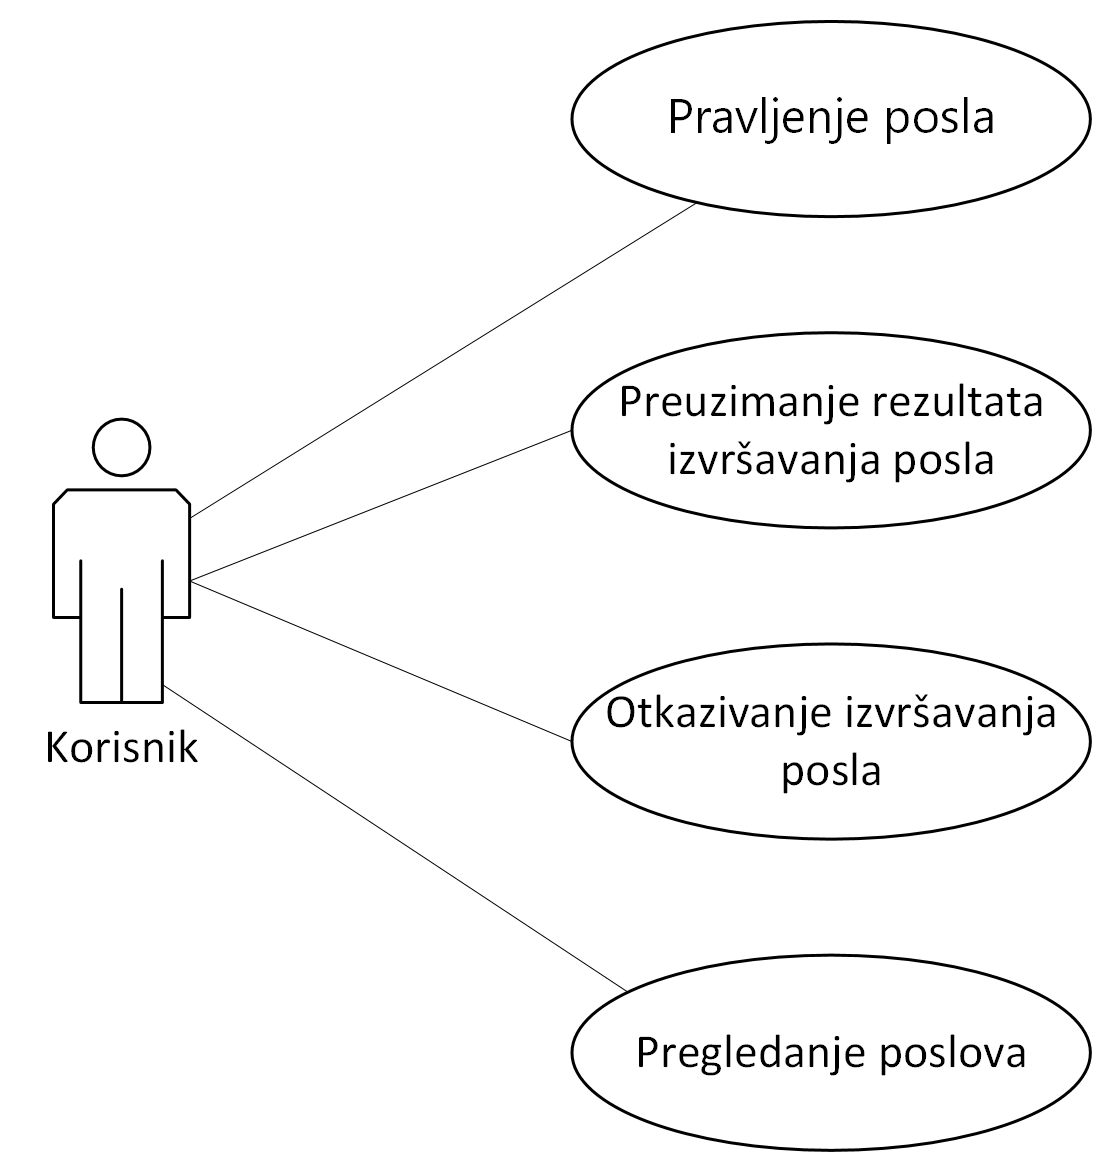
\includegraphics[width=0.6\textwidth]{./images/dijagram_slucajeva_upotrebe_korisnik.png}
  \caption{UML dijagram slučajeva upotrebe - Korisnik}
  \label{fig:slucajupotrebe_korisnik}
\end{figure}

% Zakazivanje
\subsection{Zakazivanje posla}
\begin{enumerate}
\item Naziv: Zakazivanje posla
\item Akter: Korisnik koji želi da izvrši posao nad ulaznim podacima
\item Kratak opis: Korisnik šalje zahtev za izvršavanje posla. Sistem validira zahtev i vraća potvrdu o uspešnosti zakazivanja.
\item Preduslovi: Korisnik ima pristup internetu. Korisnik ima neophodna prava da bi poslao zahtev sistemu. Sistem je u funkciji.
\item Postuslovi: Sistem je evidentirao novi zahtev za posao i prosledio ga na asinhrono izvršavanje.
\item Tok događaja:
	\begin{enumerate}
	\item \label{zak:konstruisezahtev}Korisnik konstruiše zahtev za izvršavanje posla. Zahtev se sastoji od:
		\begin{enumerate}
		\item Specifikacije tipa posla,
		\item Niza ulaznih podataka
		\end{enumerate}
	\item \label{zak:saljezahtev} Korisnik šalje zahtev sistemu preko interneta koristeći predefinisani interfejs.
	\item \label{zak:proveraprava} Sistem proverava korisnikova prava.
	\item \label{zak:validacijazahteva} Sistem validira novopridošli zahtev za izvršavanje posla.
	\item Sistem evidentira novi zahtev za izvršavanje u bazi.
	\item \label{zak:asinhzakazivanje} Sistem stavlja zahtev u red za asinhrono izvršavanje.
	\item Korisnik dobija potvrdu da je posao zakazan i identifikator po kojem je posao zaveden u sistemu.
	\end{enumerate}
\item Alternativni tok događaja:
	\begin{enumerate}
	\item Korisnik nema prava da podnese zahtev. Ukoliko u koraku \ref{zak:proveraprava} korisnik nema neophodna prava, sistem odbija zahtev uz odgovarajuću grešku. Proces se nastavlja u koraku \ref{zak:saljezahtev} glavnog toka.
	\item Zahtev je nevalidan. Ukoliko u koraku \ref{zak:validacijazahteva} sistem prepozna nevalidan zahtev, odbija ga uz odgovarajuću grešku. Nevalidan zahtev može biti:
		\begin{enumerate}
		\item Nevalidna specifikacija tipa posla. Zahtevani tip posla mora biti podržan od strane sistema,
		\item Format ulaznih podataka nije odgovarajući.
		\end{enumerate}
Proces se nastavlja u koraku \ref{zak:konstruisezahtev} glavnog toka.
	\item Sistem je preopterećen i nema dovoljno resursa da zakaže novi posao. Ukoliko u koraku \ref{zak:asinhzakazivanje} sistem proceni da nema dovoljno resursa za izvršavanje posla, on odbija zahtev uz grešku da je sistem preopterećen i da korisnik pokuša kasnije. Proces se nastavlja u koraku \ref{zak:saljezahtev} glavnog toka.
	\end{enumerate}
\item Podtokovi: /
\item Specijalni zahtevi: Korisnik ima neophodno znanje za kreiranje zahteva i korišćenje interfejsa sistema.
\item Dodatne informacije: /
\end{enumerate}

% Dohvatanje rezultata
\subsection{Preuzimanje rezultata posla}
\begin{enumerate}
\item Naziv: Preuzimanje rezultata posla
\item Akter: Korisnik koji želi da pruzme rezultate prethodno zakazanog posla
\item Kratak opis: Korisnik šalje zahtev za preuzimanje rezultata izvršavanja. Sistem validira zahtev i vraća tražene rezultate.
\item Preduslovi: Korisnik ima pristup internetu. Korisnik ima neophodna prava da bi poslao zahtev sistemu. Sistem je u funkciji. Posao je izvršen i rezultati su dostupni u bazi.
\item Postuslovi: Sistem je prosledio rezultate izvršavanja korisniku.
\item Tok događaja:
	\begin{enumerate}
	\item \label{rez:konstruisezahtev} Korisnik konstruiše zahtev za preuzimanje rezultata posla. Zahtev se sastoji od identifikatora posla za koji želi da preuzme rezultate.
	\item \label{rez:saljezahtev} Korisnik šalje zahtev sistemu preko interneta koristeći predefinisani interfejs.
	\item \label{rez:proveraprava} Sistem proverava korisnikova prava.
	\item \label{rez:validacijazahteva} Sistem validira novopridošli zahtev za preuzimanje rezultata posla.
	\item \label{rez:sinhslanjerez} Sistem šalje rezultate korisniku.
	\item Korisnik dobija rezultate.
	\end{enumerate}
\item Alternativni tok događaja:
	\begin{enumerate}
	\item Korisnik nema prava da podnese zahtev. Ukoliko u koraku \ref{rez:proveraprava} korisnik nema neophodna prava, sistem odbija zahtev uz odgovarajuću grešku. Proces se nastavlja u koraku \ref{rez:saljezahtev} glavnog toka.
	\item Zahtev je nevalidan. Ukoliko u koraku \ref{rez:validacijazahteva} sistem prepozna da posao sa datim identifikatorom ne postoji, odbija zahtev uz odgovarajuću grešku. Proces se nastavlja u koraku \ref{rez:konstruisezahtev} glavnog toka.
	\end{enumerate}
\item Podtokovi: /
\item Specijalni zahtevi: Korisnik ima neophodno znanje za generisanje zahteva i korišćenje interfejsa sistema.
\item Dodatne informacije: Ukoliko je posao uspešno izvršen, rezultat izvršavanja se sastoji od traženog rezultata izračunavanja. Ukoliko je posao neuspešno obrađen, rezultat se sastoji od informacije o grešci.
\end{enumerate}

% Otkazivanje
\subsection{Otkazivanje posla}
\begin{enumerate}
\item Naziv: Otkazivanje posla
\item Akter: Korisnik koji želi da otkaže prethodno zakazani posao
\item Kratak opis: Korisnik šalje zahtev za otkazivanje posla. Sistem validira zahtev i vraća potvrdu o uspešnosti otkazivanja.
\item Preduslovi: Korisnik ima pristup internetu. Korisnik ima neophodna prava da bi poslao zahtev sistemu. Sistem je u funkciji.
\item Postuslovi: Sistem je otkazao posao i azurirao evidenciju posla u bazi.
\item Tok događaja:
	\begin{enumerate}
	\item \label{otk:konstruisezahtev} Korisnik konstruiše zahtev za otkazivanje posla. Zahtev se sastoji od identifikatora posla koji želi da otkaže.
	\item \label{otk:saljezahtev} Korisnik šalje zahtev sistemu preko interneta koristeći predefinisani interfejs.
	\item \label{otk:proveraprava} Sistem proverava korisnikova prava.
	\item \label{otk:validacijazahteva} Sistem validira novopridošli zahtev za otkazivanje posla.
	\item \label{otk:sinhotkazivanje} Sistem sinhrono otkazuje sve operacije povezane sa poslom.
	\item Korisnik dobija potvrdu da je posao otkazan.
	\end{enumerate}
\item Alternativni tok događaja:
	\begin{enumerate}
	\item Korisnik nema prava da podnese zahtev. Ukoliko u koraku \ref{otk:proveraprava} korisnik nema neophodna prava, sistem odbija zahtev uz odgovarajuću grešku. Proces se nastavlja u koraku \ref{otk:saljezahtev} glavnog toka.
	\item Zahtev je nevalidan. Ukoliko u koraku \ref{otk:validacijazahteva} sistem prepozna da posao sa datim identifikatorom ne postoji ili nije aktivan, odbija zahtev uz odgovarajuću grešku. Proces se nastavlja u koraku \ref{otk:konstruisezahtev} glavnog toka.
	\end{enumerate}
\item Podtokovi: /
\item Specijalni zahtevi: Korisnik ima neophodno znanje za generisanje zahteva i korišćenje interfejsa sistema.
\item Dodatne informacije: /
\end{enumerate}

% Pregled poslova
\subsection{Pregled poslova}
\begin{enumerate}
\item Naziv: Pregled poslova
\item Akter: Korisnik koji želi da pruzme listu evidentiranih poslova u sistemu.
\item Kratak opis: Korisnik šalje zahtev za izlistavanje evidentiranih poslova. Sistem validira zahtev i vraća tražene informacije o evidentiranim poslovima.
\item Preduslovi: Korisnik ima pristup internetu. Korisnik ima neophodna prava da bi poslao zahtev sistemu. Sistem je u funkciji. Posao je izvršen i rezultati su dostupni u bazi.
\item Postuslovi: Sistem je prosledio rezultate izvršavanja korisniku.
\item Tok događaja:
	\begin{enumerate}
	\item \label{pregledp:konstruisezahtev} Korisnik konstruiše zahtev za izlistavanje poslova.
	\item \label{pregledp:saljezahtev} Korisnik šalje zahtev sistemu preko interneta koristeći predefinisani interfejs.
	\item \label{pregledp:proveraprava} Sistem proverava korisnikova prava.
	\item \label{pregledp:slanjeliste} Sistem šalje listu evidentiranih poslova dostupnih u bazi.
	\item Korisnik dobija listu evidentiranih poslova.
	\end{enumerate}
\item Alternativni tok događaja:
	\begin{enumerate}
	\item Korisnik nema prava da podnese zahtev. Ukoliko u koraku \ref{pregledp:proveraprava} korisnik nema neophodna prava, sistem odbija zahtev uz odgovarajuću grešku. Proces se nastavlja u koraku \ref{pregledp:saljezahtev} glavnog toka.
	\end{enumerate}
\item Podtokovi: /
\item Specijalni zahtevi: Korisnik ima neophodno znanje za generisanje zahteva i korišćenje interfejsa sistema.
\item Dodatne informacije: Rezultujuća lista poslova sadrži informacije o svakom evidentiranom poslu, i to:
	\begin{enumerate}
	\item Identifikator posla
	\item Status posla
	\item Vreme početka zvršavanja posla
	\item Vreme završetka izvršavanja posla
	\end{enumerate}
\end{enumerate}

% Administratorovi slučajevi upotrebe
\section{Podešavanje sistema}
Dodatne funkcionalnosti sistema uključuju slučajeve upotrebe u kojima je učesnik administrator. Ovo uključuje podešavanje bezbednosti i prava pristupa sistemu, kao i prilagođavanje sistema da bude u u skladu sa korisnikovim korišćenjem, tj. opterećenosti sistema.

% Pristup podacima je ograničen i neophodno je da mogu da im pristupe samo autorizovane osobe.  -- prebaci negde

% AAD Admin
\subsection{Podešavanja prava pristupa}
Prava pristupa sistemu, tj. delovima sistema dodeljuje administrator za bezbednost. Prava pristupa pojedinačnim delovima sistema se kontrolišu kroz različta prava koja mogu biti dodeljena korisniku. Tipovi prava su:
	\begin{enumerate}
	\item Iskustvo krajnjeg korisnika - Mogućnost slanja zahteva sistemu kroz definisani javni interfejs,
	\item Pravo za praćenje rada sistema - Pristup telemetriji i logovima za praćenje rada sistema,
	\item Administrator klastera - Pristup klasteru za devops akcije,
	\item Administrator bezbednosti.
	\end{enumerate}
Slučajevi upotrebe iz ugla administratora za bezbednost su prikazani na slici \ref{fig:slucajupotrebe_aadadmin}. Ovih slučajevi upotrebe su jednostavni i intuitivni, te nisu opisani u nastavku.

\begin{figure}[!ht]
  \centering
  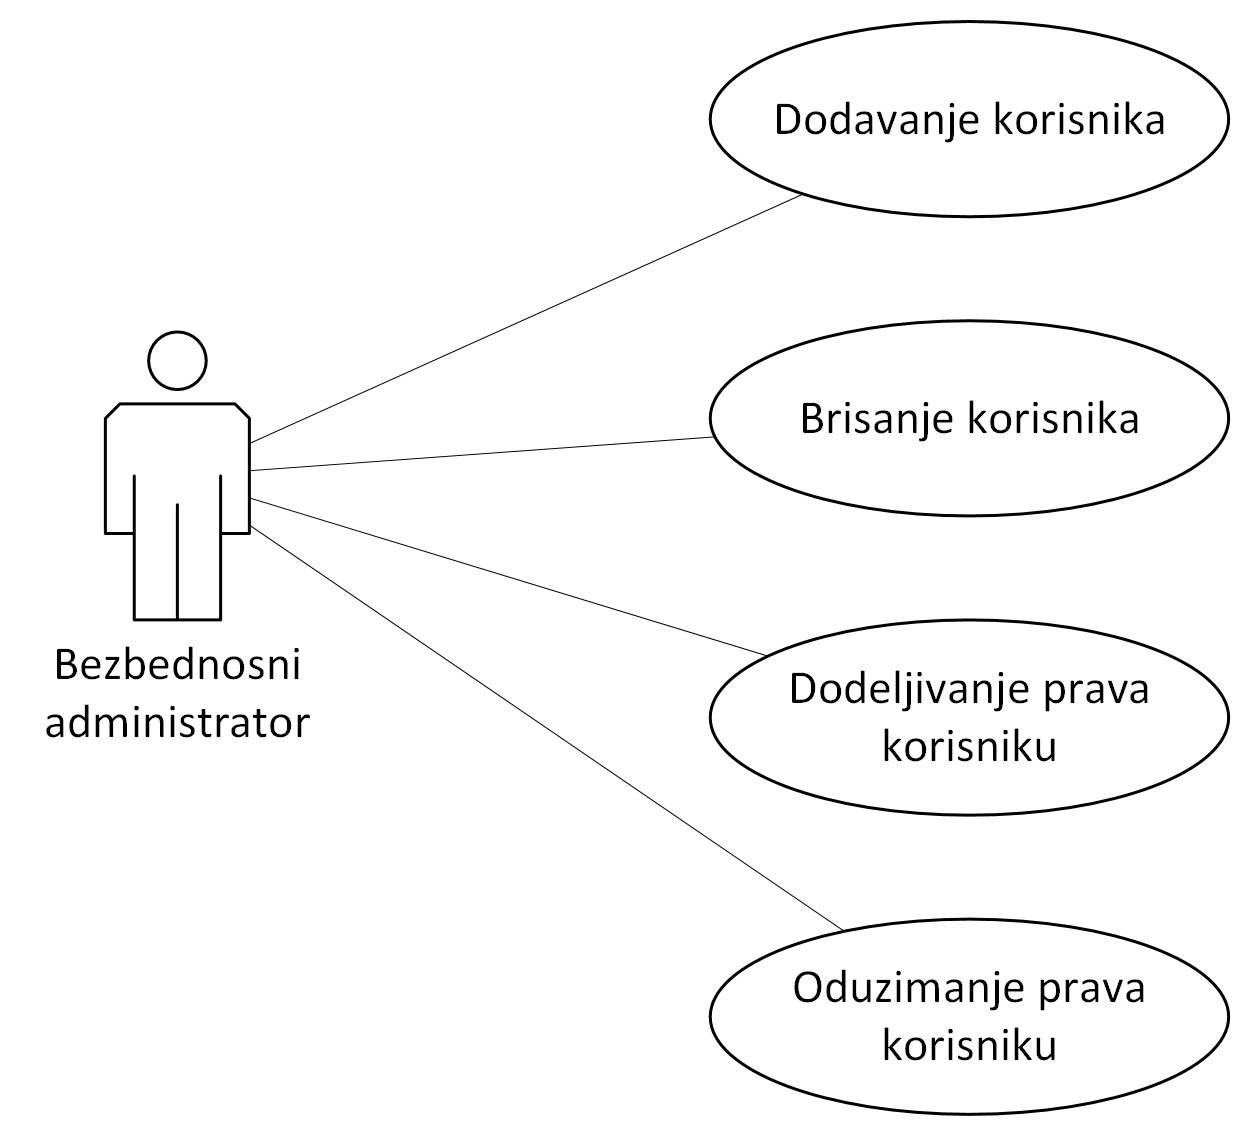
\includegraphics[width=0.6\textwidth]{./images/dijagram_slucajeva_upotrebe_administrator_sistema_aadadmin.png}
  \caption{UML dijagram slučajeva upotrebe - Administrator za bezbednost}
  \label{fig:slucajupotrebe_aadadmin}
\end{figure}


% Podešavanje AKS klastera
\subsection{Podešavanje klastera}
Klaster administrator ima mogućnost da menja konfiguraciju sistema kako bi ga prilagodio potrebama krajnjeg korisnika. To uključuje horizontalno i vertikalno skaliranje sistema. Horizontalno skaliranje sistema podrazumeva menjanje broja pokrenutih servisa koji se koriste tokom izvršavanja posla. Vertikalno skaliranje podrazumeva ažuriranje konfiguracije kojom se dodeljuju resursi servisima (dostupna memorija i procesorsko vreme).

Slučajevi upotrebe iz ugla klaster administratora su prikazani na slici \ref{fig:slucajupotrebe_admin_klastera}. Detalji ovih slučajeva upotrebe su konceptualno jasni, a uključuju poznavanje implementacionih detalja, te nisu dalje razrađivani.

\begin{figure}[!ht]
  \centering
  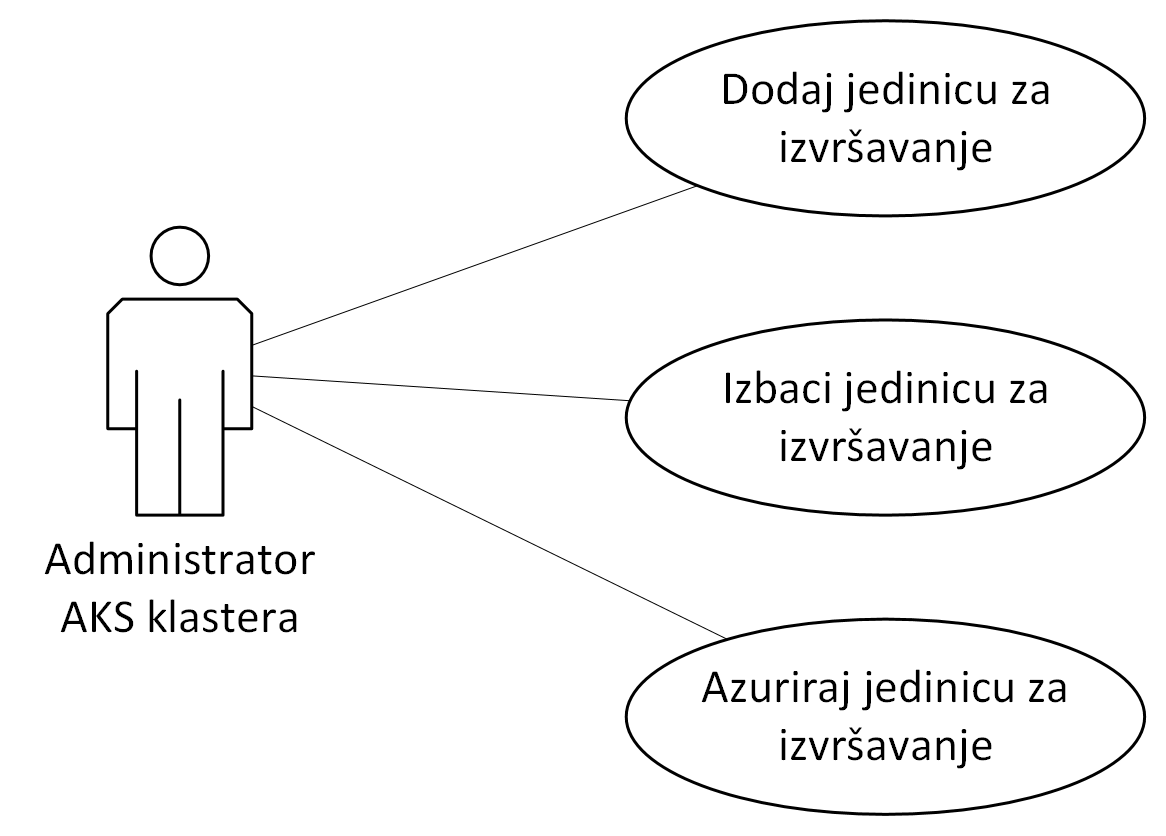
\includegraphics[width=0.6\textwidth]{./images/dijagram_slucajeva_upotrebe_administrator_klastera.png}
  \caption{UML dijagram slučajeva upotrebe - Klaster administrator}
  \label{fig:slucajupotrebe_admin_klastera}
\end{figure}

% ------------------------------------------------------------------------------
\chapter{Opis korišćenih tehnologija i alata}
\label{chp:opistehialata}
% ------------------------------------------------------------------------------

U ovom poglavlju biće opisane tehnologije i alati korišćenih prilikom programske realizacije sistema.
Za implementaciju je korišćen programski jezik C\#, i \emph{.NET Core 6.0} radni okvir. Korišćeno razvojno okruženje je \emph{Microsoft Visual Studio Community 2022} i operativni sistem \emph{Windows 10}.

\section{Doker platforma}
Za pokretanje aplikacija je korišćena Doker platforma (eng. \emph{Docker}) \cite{Docker}. Prednosti korišćenja ove platforme su monogstuke. Za početak, ona razdvaja razvijanje aplikacije od infrastrukture na kojoj će biti pokrenuta. Aplikacija je spakovana u izolovano okruženje koje se naziva kontejner (eng. \emph{container}). Kontejneri sadrže sve (a u idealnom slučaju, samo) ono što je neophodno za pokretanje aplikacije, u vidu strukture koja se naziva slika (eng. \emph{image}). To čini da su kontejneri lagani za prenošenje, za razliku od virtuelnih mašina koje u teoriji mogu pružiti istu funkcionalnost. Spakovana aplikacija može biti pokrenuta neograničeni broj puta, u različitim okruženjima: prilikom ručnog i automatskog testiranja, u produkciji, itd. Prilikom pokretanja kontejnera, može se dodatno specificirati njegova konfiguracija (na primer, mapiranje portova).

Arhitektura platforme je predstavljena na slici \ref{fig:dockerarch}, preuzetoj iz zvanične dokumentacije \cite{DockerArch}. 

\begin{figure}[!ht]
  \centering
  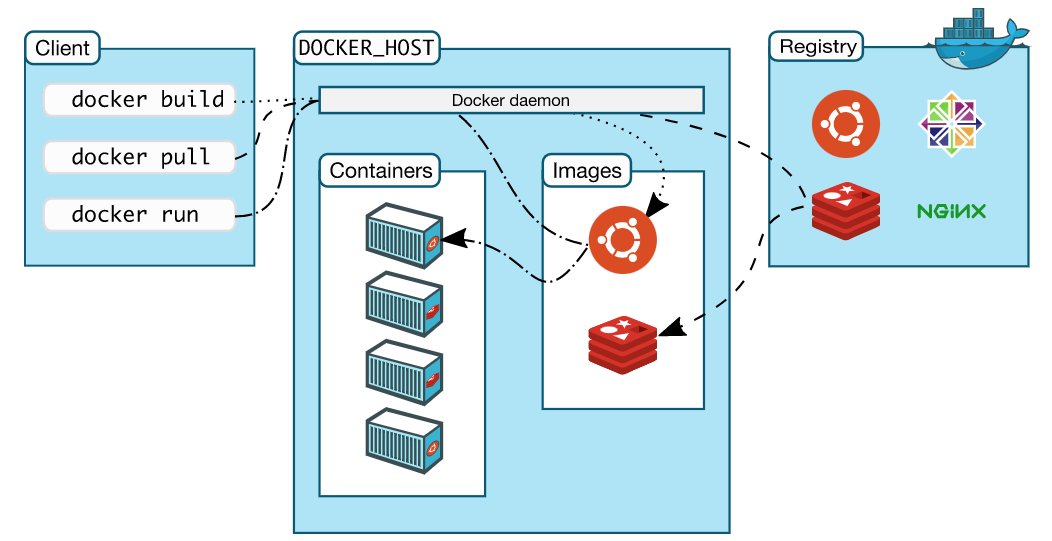
\includegraphics[width=1.0\textwidth]{./images/docker_architecture.png}
  \caption{Arhitektura Doker platforme}
  \label{fig:dockerarch}
\end{figure}

Koraci potrebni da se napravi slika aplikacije se definišu u \emph{Dockerfile} datoteci. Svaka instrukcija u ovom fajlu kreira sloj slike (eng. \emph{layer}). U sličaju \emph{.NET Core} aplikacija, prvi korak je učitavanje željenog radnog okvira, zatim, (primera radi) pokretanje kompilacije izvornog koda i smeštanje izvršnog koda na željenu lokaciju. Krajnji korak je uglavnom definisanje komande za pokretanje aplikacije. Bitno je naglasiti da tokom razvijanja aplikacije, Doker prepoznaje koji slojevi slike koji su se promenili, te ponovo kreira samo njih i njihove naredne slojeve. Ovo čini generisanje slike efikasnom i brzom operacijom koja ne usporava programera, koji najčeće menja samo delove aplikacije. Kreirane slike se čuvaju u registru slika koji može biti lokalni ili negde u oblaku.

Kontejner sadrži specifikaciju operativnog sistema na kojem se pokreće slika. Izbor \emph{.NET Core} radnog okvira omogućava pokretanje servisa na različitim platformama \emph{Windows}, \emph{Mac} i \emph{Linux}, bez izmena izvornog koda. Za izradu sistema su korišćeni \emph{Linux} kontejneri.

Korišćeno okruženje za lokalno kreiranje i pokretanje kontejnera je \emph{Docker Desktop} prikazan na slici \ref{fig:dockerdesktop}.

\begin{figure}[!ht]
  \centering
  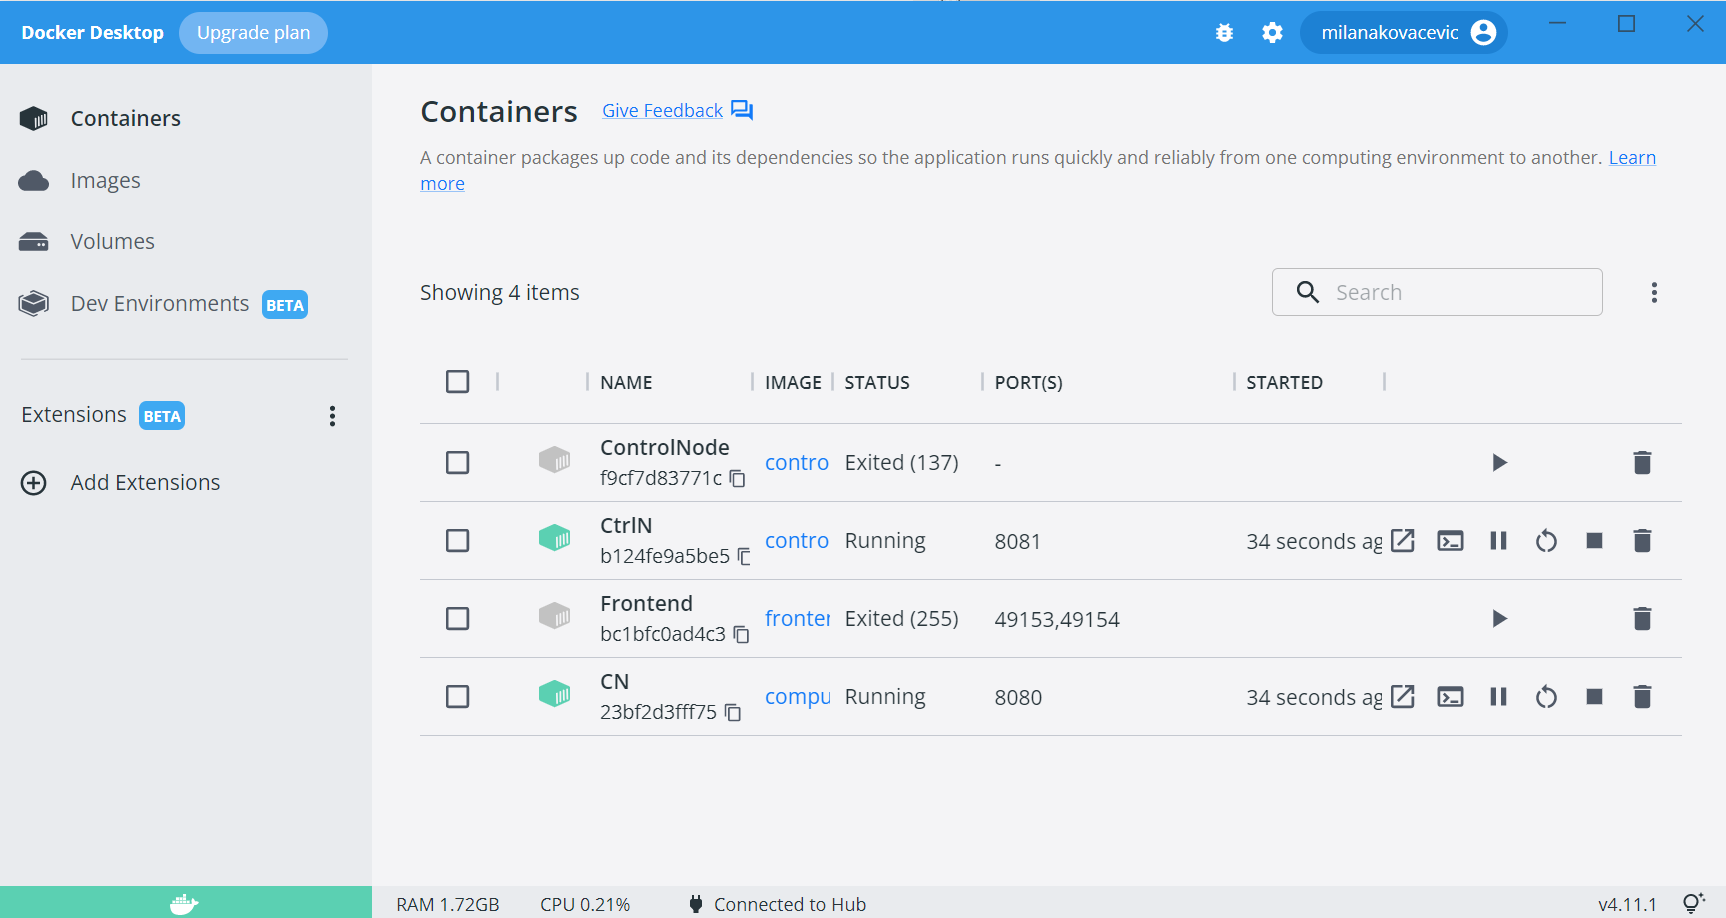
\includegraphics[width=1.0\textwidth]{./images/docker_desktop.png}
  \caption{Docker Desktop}
  \label{fig:dockerdesktop}
\end{figure}

% Kubernetes detalji
\section{Kubernetes platforma}

Pokretanje sistema na praktičan i skalabilan način, omogućila je \emph{Kubernetes} platforma \cite{Kubernetes}. Ona pruža potrebnu infrastrukturu za pokretanje aplikacija zapakovanih u Doker kontejnere, kao i za upravljanje njima i ostalim pratećim delovima sistema.

Kubenetes omogućava:
\begin{enumerate}
\item Pronalaženje servisa koristeći DNS ime ili IP adresu,
\item Balansiranje saobraćaja kroz mrežu u zavisnosti od opterećenosti,
\item Korišćenje diska i drugih skladišta podataka,
\item Automatsko ažuriranje (eng. \emph{update}) verzija aplikacije kao i vraćanje na prethodnu verziju,
\item Upravljanje resursima i pakovanje kontejnera na mašine,
\item \emph{Self-healing} - automatski restart kontejnera koji ne ispunjavaju uslove zrdravlja,
\item Upravljanje konfiguracijom, šiframa, sertifikatima i drugim osetljivim informacijama - uz samostalno ažuriranje bez potrebe za promenom slike kontejnera.
\end{enumerate}

Na slici \ref{fig:kubernetesarh} prikazana je arhitektura Kubernetes klastera, preuzeta iz zvanične dokumentacije \cite{KubernetesArchitecture}.

\begin{figure}[!ht]
  \centering
  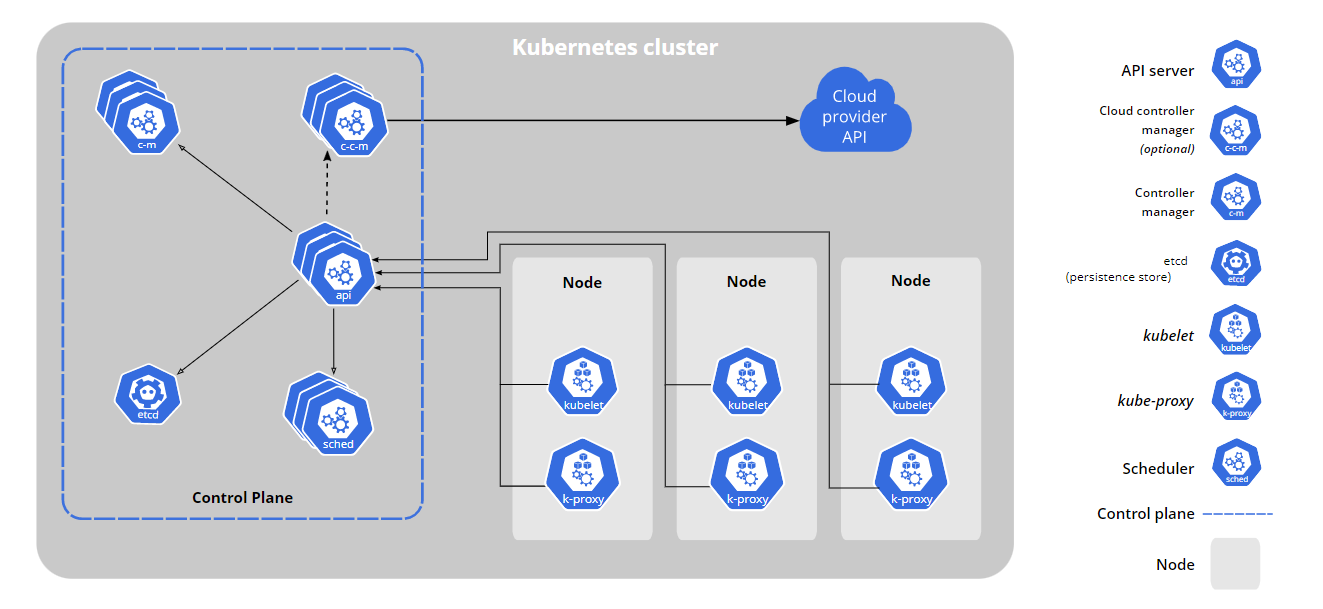
\includegraphics[width=1.0\textwidth]{./images/kubernetes_architecture.png}
  \caption{Arhitektura Kubernetes klastera}
  \label{fig:kubernetesarh}
\end{figure}

Kubernetes klaster se sastoji iz dve celine: kontrolnog dela i skupa radnih mašina (eng. \emph{nodes}). Radne mašine na sebi pokreću \emph{mahune} (eng. \emph{pod}) u okviru kojih je smešten jedan ili više kontejner, u okviru kojih se nalazi aplikacija. \emph{Pod} je najmanja jedinica koju je moguće kreirati i pokrenuti na klasteru, a kontejneri unutar njega imaju istu specifikaciju i dele lokalnu mrežu.

Kako bi pokrenute aplikacije bile dostupne na mreži, kreira se apstrakcija koja se naziva \emph{Servis}. Ova apstrakcija povezuje grupu \emph{pod}ova i definiše način na koji im se pristupa: koristeći jedinstveno DNS ime ili IP adresu (eng. \emph{Service endpointa}). Slanjem poruka na ovu adresu, Kubernetes sam usmerava i balansira saobraćaj ka \emph{pod}ovima, od kojih svaki ima jedinstvenu IP adresu.

U okviru svake radne mašine je pokrenuto još nekoliko sistemskih procesa: 
\begin{enumerate}
\item \emph{kuberlet} - Zadužen za pokretanje kontejnera na mašini, kao i za praćenje rada kontejnera i njegovog zdravlja.
\item \emph{kube-proxy} - Zadužen za podešavanje pravila mreže koja omogućavaju slanje i prijem poruka \emph{pod}ovima, koristeći specifikacije definisane servisima.
\item \emph{Container runtime} - Zadužen za pokretanje kontejnera.
\end{enumerate}

Kontrolni deo klastera služi za upravljanje klasterom, a funkcionalnosti su obezbeđene kroz nekoliko komponenti:
\begin{enumerate}
\item \emph{kube-apiserver} - Server API koji prima zahteve upućene klasteru.
\item \emph{etcd} - Služi za skladište podatka u klasteru.
\item \emph{kube-scheduler} - Zadužen za smeštanje novih \emph{pod}-ova na mašine u skladu sa dostupnim i traženim resursima, kao i drugim specifikacijama (na primer, međusobni afinitet servisa).
\item \emph{kube-controller-manager} - Sastoji se od nekoliko kontrolera:
	\begin{enumerate}
	\item \emph{node-controller} - Omogućava reagovanje u slučajevima kada mašine postanu nedostupne.
	\item \emph{job-controller} - Izvšava dodatne poslove na klasteru.
	\item \emph{endpoints-controller} - Podešava endpointe, tj. omogućava pronalaženje servisa i \emph{pod}ova koje obuhvata. Ažurira adrese u slučaju promena (dodavanja i brisanja \emph{pod}ova).
	\item \emph{Servce Account \& Token Controller} - Resursi u okviru klastera se mogu podeliti po imenskim prostoima (eng. \emph{namespace}). Ovi kontroleri omogućavaju podešavaju prava pristupa u okviru imenskih prostora.
	\end{enumerate}
\item \emph{cloud-controller-manager} - Predstavlja vezu između klastera i cloud providera.
\end{enumerate}
Sve aplikacije su pokrenute na fizičkim mašinama koje su date na raspolaganju klasteru tokom njegovog kreiranja ili ažuriranja. Neki kontejneri/podovi mogu biti pokrenuti na istoj mašini, ali to zavisi od potražnje i raspodele resursa, kao i od drugih specifikacija. Jedna od prednosti Kubernetesa je što on vodi računa o tome gde je koji proces pokrenut, te pokušava da obezbedi najbolju otpornost na greške u sistemu (na primer, restartovanje mašine) i time obezbedi visoku dostupnost pokrenutih servisa.

Za definisanje resursa i njihovih specifikacija, kao i konfiguracije na klasteru koriste se datoteke sa ekstenzijom \emph{yaml}. Prosleđivanjem ovih datoteka klasteru se prave promene na klasteru.

Za komunikaciju sa kontrolnim delom Kubernetes klastera se koristi kilijent \emph{kubectl}. Neke od komandi su predstavljene u nastavku.

\begin{verbatim}
// Opšti oblik komande
kubectl [command] [TYPE] [NAME] [flags]
// Kreiranje resursa i njihovih specifikacija definisane u deploy.yaml
kubectl apply -f deploy.yaml
// Izlistavanje servisa na klasteru
kubectl get svc
// Izlistavanje podova
kubectl get pods
// Pristup bash konzoli na mašini u okviru koje je pokrenut pod
kubectl exec mypod-m96mk -it mypod-m96mk  -- /bin/bash
\end{verbatim}

\section{Azure platforma}

Programska implementacija sistema je uključila njegovo pokretanje u oblaku, a za to je korišćena platforma \emph{Microsoft Azure} \cite{Azure}. Ova platforma pruža veliki broj softverskih i infrastrukturnih rešenja, kao i propratnih servisa i mogućnosti koje poboljšavaju celokupno iskustvo korišćenja.

Najrelevantniji resursi korišćeni za pokretanje sistema u na \emph{Azure} platformi su:
\begin{enumerate}
\item \emph{Azure Kubernetes Service} \cite{AKS} - Resurs koji predstavlja \emph{Kubernetes} klaster.
\item \emph{Azure SQL Database} \cite{AzureSQLDB} - Resurs koji predstavlja relacionu bazu podataka.
\item \emph{Azure Active Directory} \cite{AAD} - Resurs koji omogućava kreiranje identiteta (npr. korisnike, grupe) i njihovo njegovo podešavanje (prava pristupa, login...).
\item \emph{Azure Monitor} \cite{AzureMonitor} - Skup propratnih funkcionalnosti koje pružaju uvid u ponašanje Azure resursa. Sakuplja logove i metrike, daje alate za njihovo analiziranje, kao i mogućnost uzbunjivanja (eng. \emph{alerts}) i reagovanja na dešavanja od interesa. Ima podršku i za tehnike mašinskog učenja nad sakupljenim podacima.
\end{enumerate}

\section{Dodatni alati}

\subsection{Swagger / OpenAPI}

\emph{OpenAPI} \cite{OpenAPI} je specifikacija \emph{REST API}-a koja ne zavisi od programskog jezika. \emph{Swagger} \cite{Swagger} predstavlja skup alata koji koriste \emph{OpenAPI} specifikaciju.

Servisi kreirani u okviru sistema imaju otvoreni web \emph{REST API}. Korišćenjem \emph{Swagger} skupa alata su oni dokumentovani u standardizovanom formatu, u \emph{json} datoteci. Za generisanje ove specifikacije za \emph{.NET Core} aplikacije koristi se \emph{Swashbuckle} \cite{Swashbuckle} alat.

Sa klijentske strane, koristi se alat \emph{NSwag} \cite{NSwag}. Na osnovu prethodno generisane \emph{json} datoteke, on ž tokom kompilacije generiše klasu koja sadriži \emph{HTTP} klijenta i potrebnu dokumentaciju. Ovo je praktičan i efikasan način da se automatski generiše kod klijenta pomoću kojeg se šalju zahtevi servisima sistema.

% ------------------------------------------------------------------------------
\chapter{Implementacija}
\label{chp:impl}
% ------------------------------------------------------------------------------

U ovom poglavlju biće opisana implementacija sistema (eng. \emph{Distributed Computation System}).
Projekat je javno dostupan na servisu GitHub na adresi \href{https://github.com/milana-kovacevic/DistributedComputationSystem}{https://github.com/milana-kovacevic/DistributedComputationSystem}. Na adresi se takođe nalaze datoteke potrebne za kreiranje i konfiguraciju servisa pokrenutih u okviru Kubernetes klastera, kao i pomoćne skripte koje automatizuju proces postavljanja nove verzije aplikacija na klaster.


\section{Arhitektura sistema}

Arhitektura sistema je prikazana na slici \ref{fig:arhitektura}.

\begin{figure}[!ht]
  \centering
  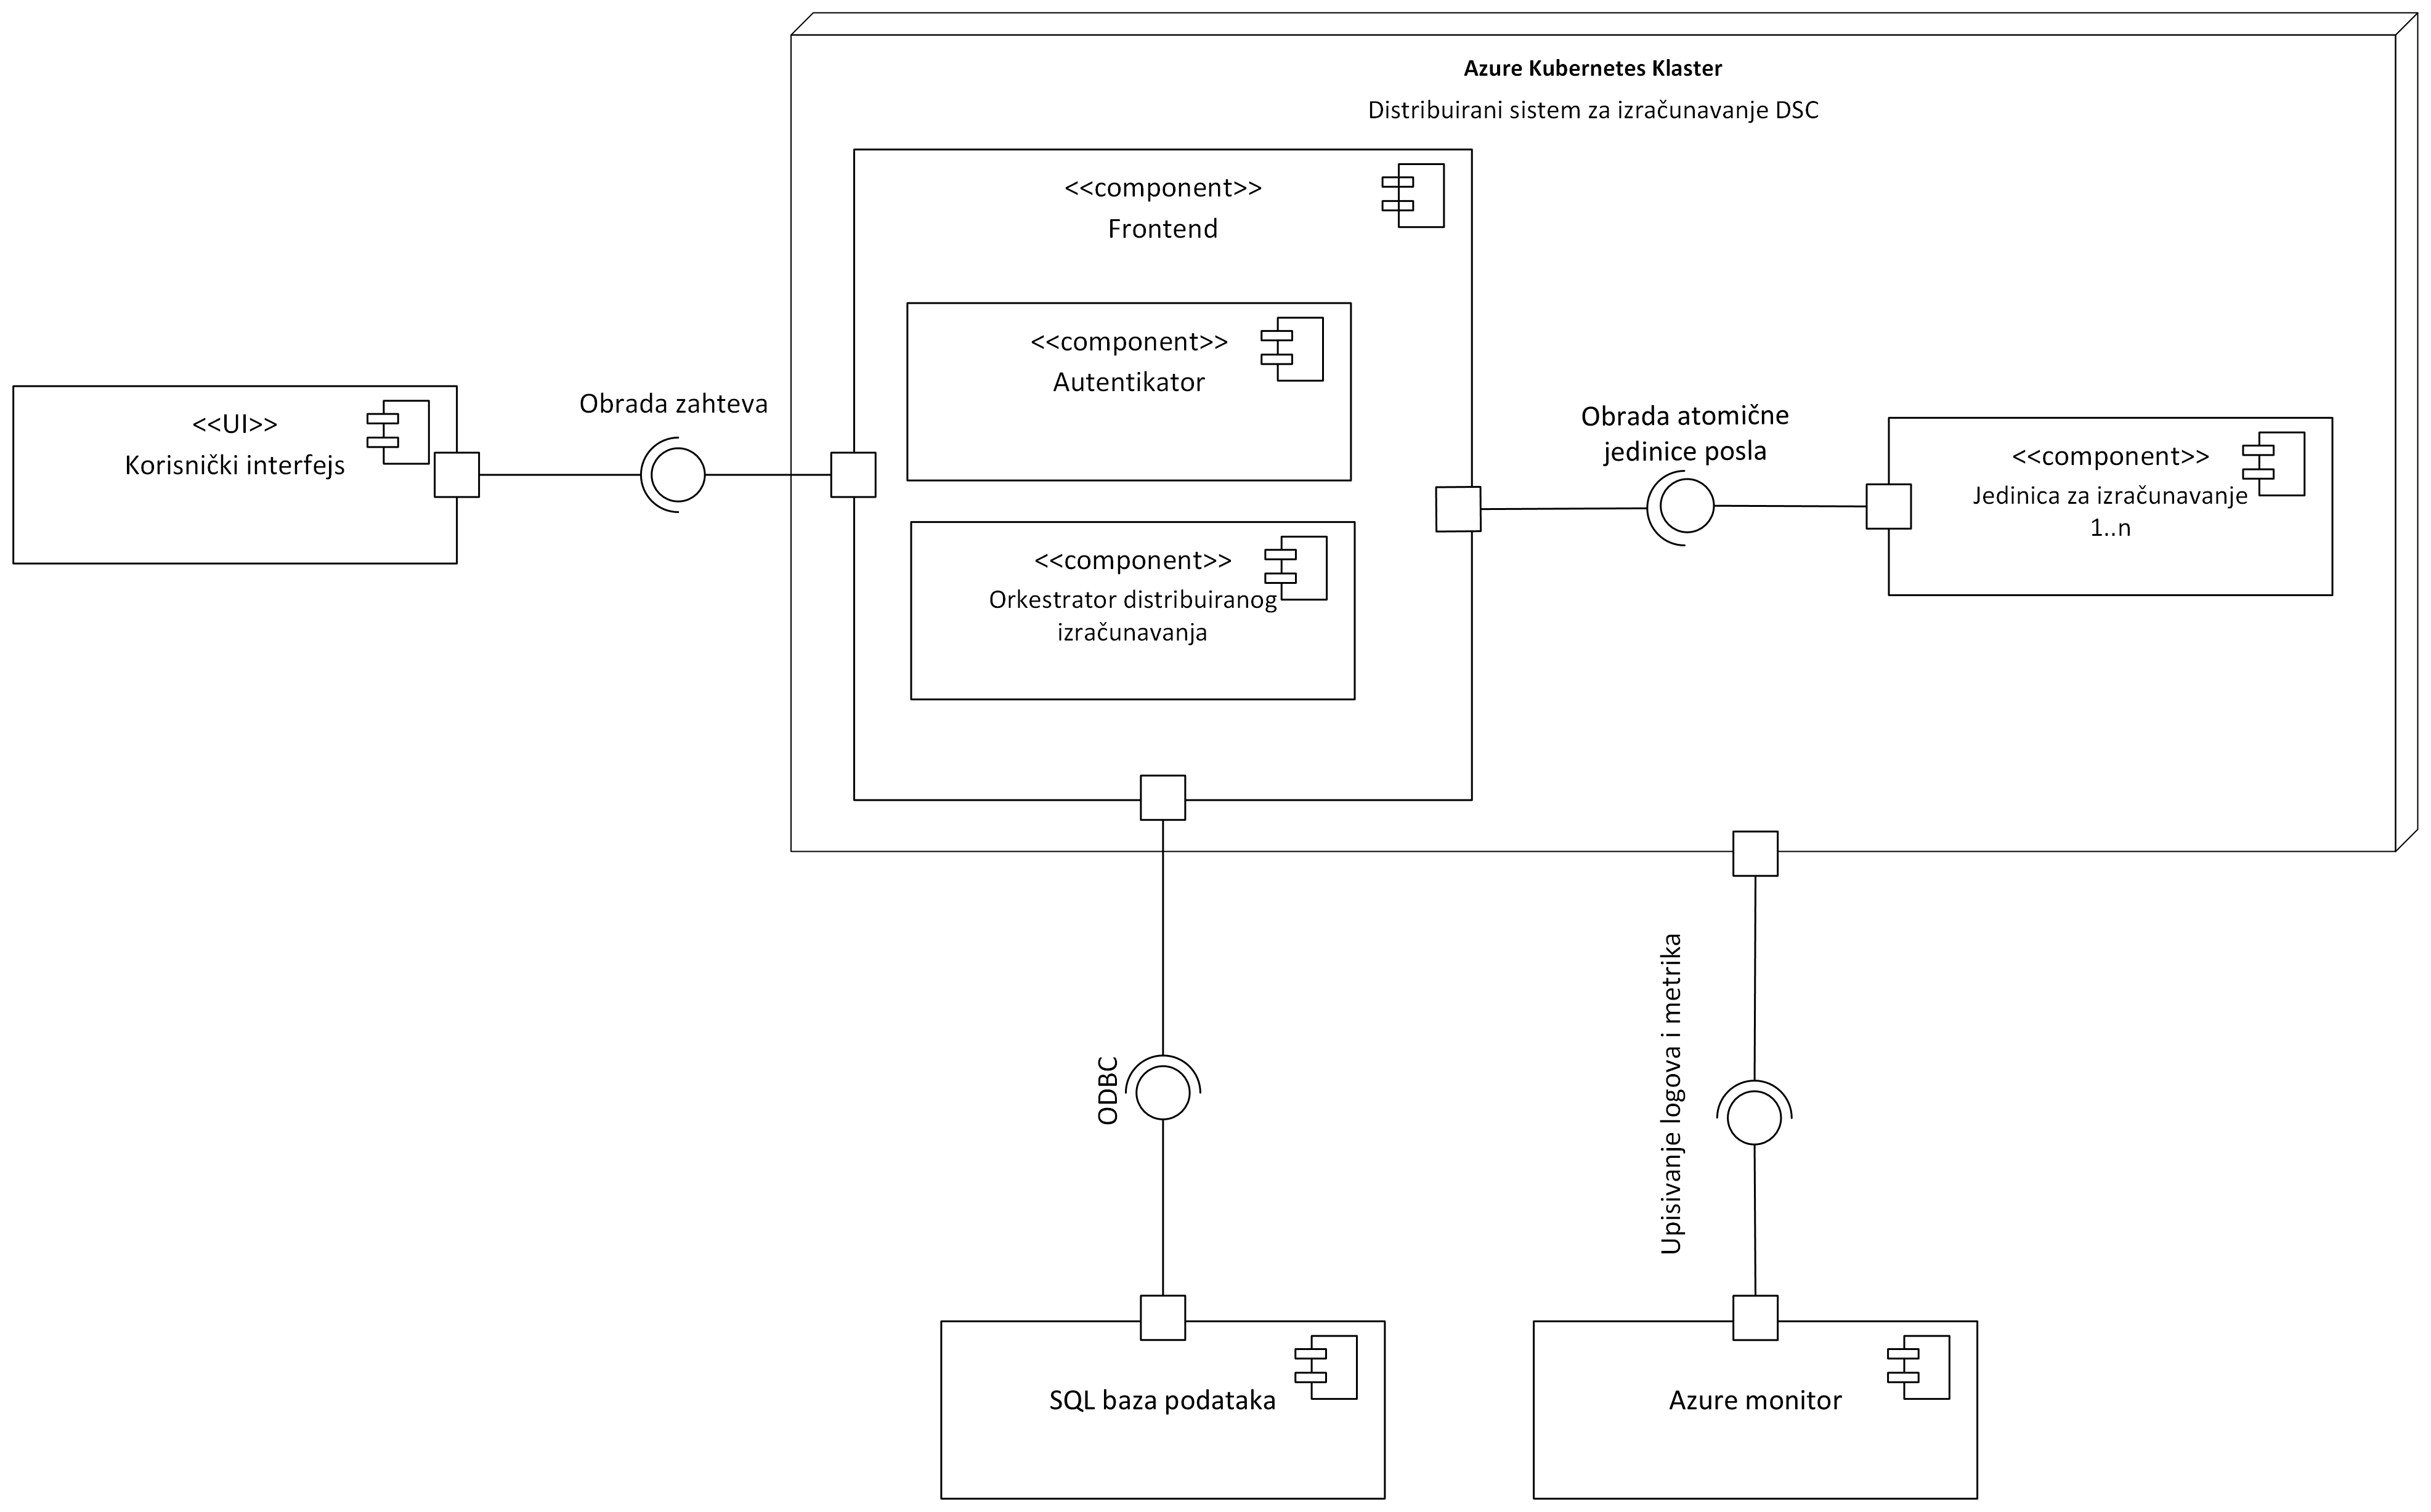
\includegraphics[width=1.0\textwidth]{./images/arhitektura_sistema_dijagram_komponenti.png}
  \caption{UML dijagram komponenti - Arhitektura sistema}
  \label{fig:arhitektura}
\end{figure}

Arhutekturalni obrazac korišćen prilikom razvoja pojedinačnih servisa sistema (Frontenda i Jedinice za izračunavanje) je Model-Pogled-Kontroler (eng. \emph{Model-View-Controller}), bez implementacije Pogled dela. Razlog za odabir ovog obrasca je što on uvodi podelu odgovornosti različitih delova servisa. Kontroler je okrenut ka spolja, i definiše interfejs za komunikaciju sa servisom. U slučaju Frontenda, on definiše API (eng. \emph{Application Programming Interface}) koji prima korisnikove zahteve za izvršavanje posla.

\section{Autentikacija}

Proces autentikacije je prikazan na slici \ref{fig:autentikacija}.

\begin{figure}[!ht]
  \centering
  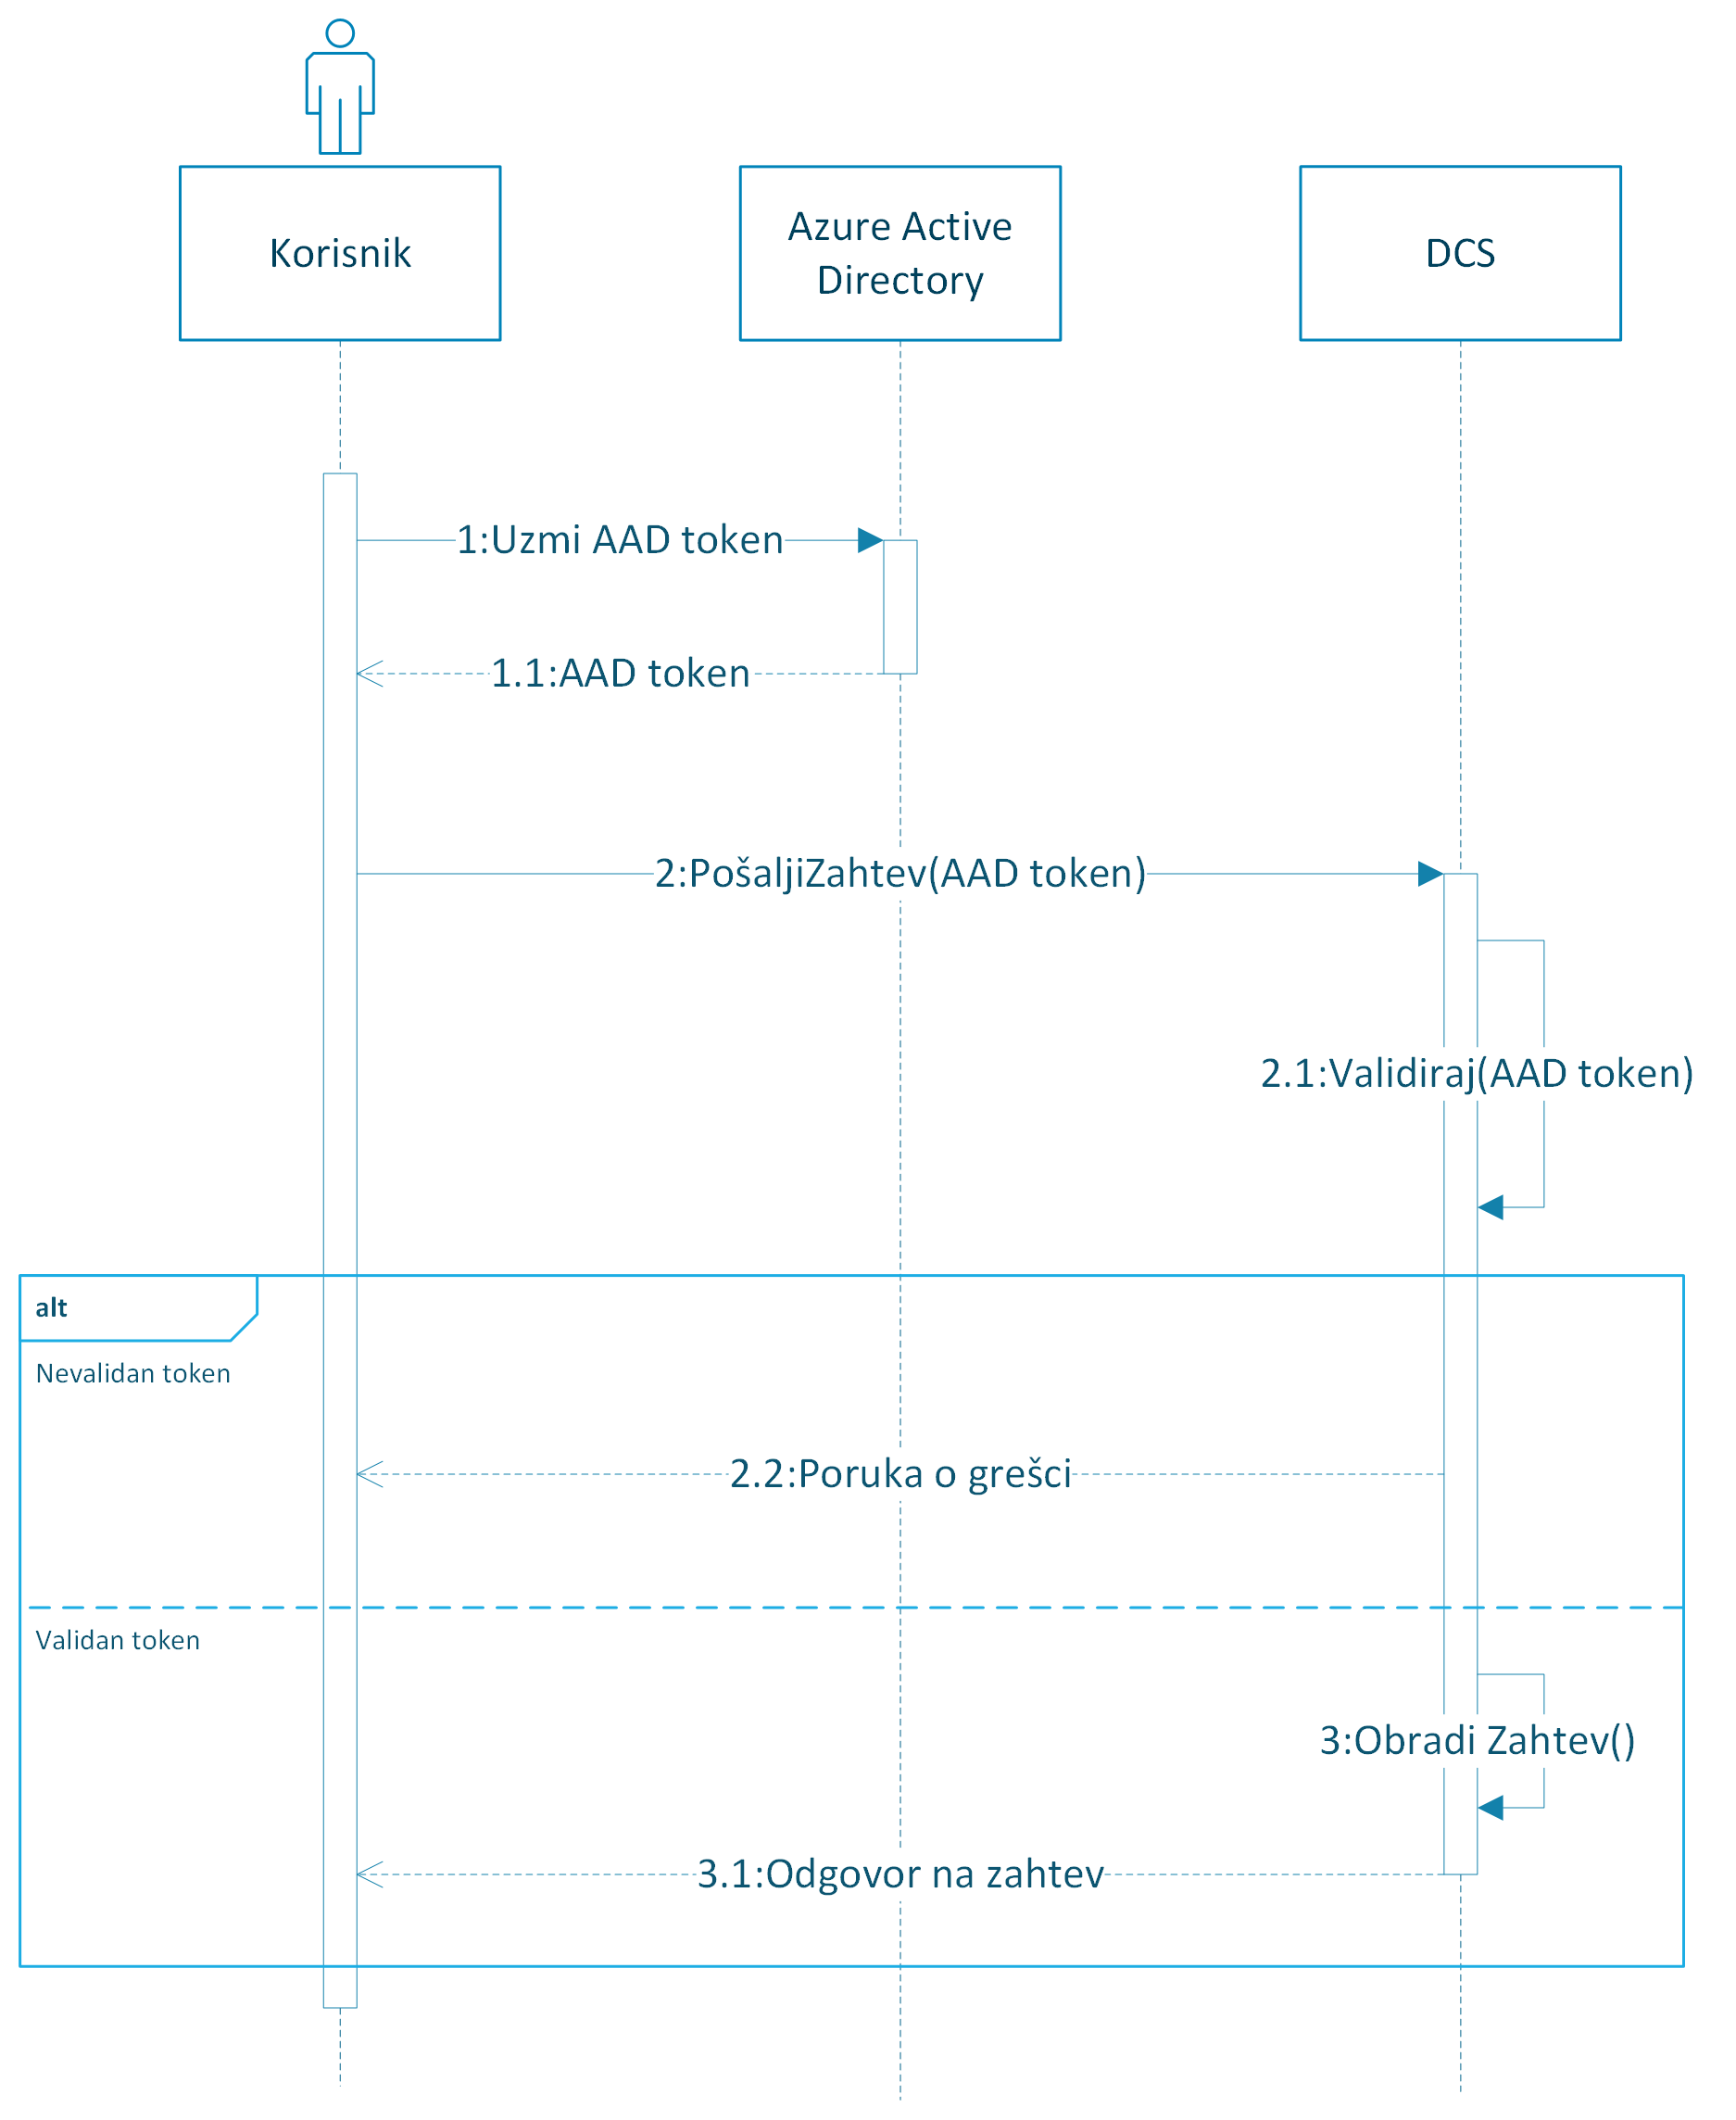
\includegraphics[width=1.0\textwidth]{./images/autentikacija_uml_dijagram_sekvence.png}
  \caption{UML dijagram sekvence - Autentikacija}
  \label{fig:autentikacija}
\end{figure}


\section{Baza}

ER (eng. \emph{Entity-Relation}) dijagram modela posla je prikazanan na slici \ref{fig:erposao}.

\begin{figure}[!ht]
  \centering
  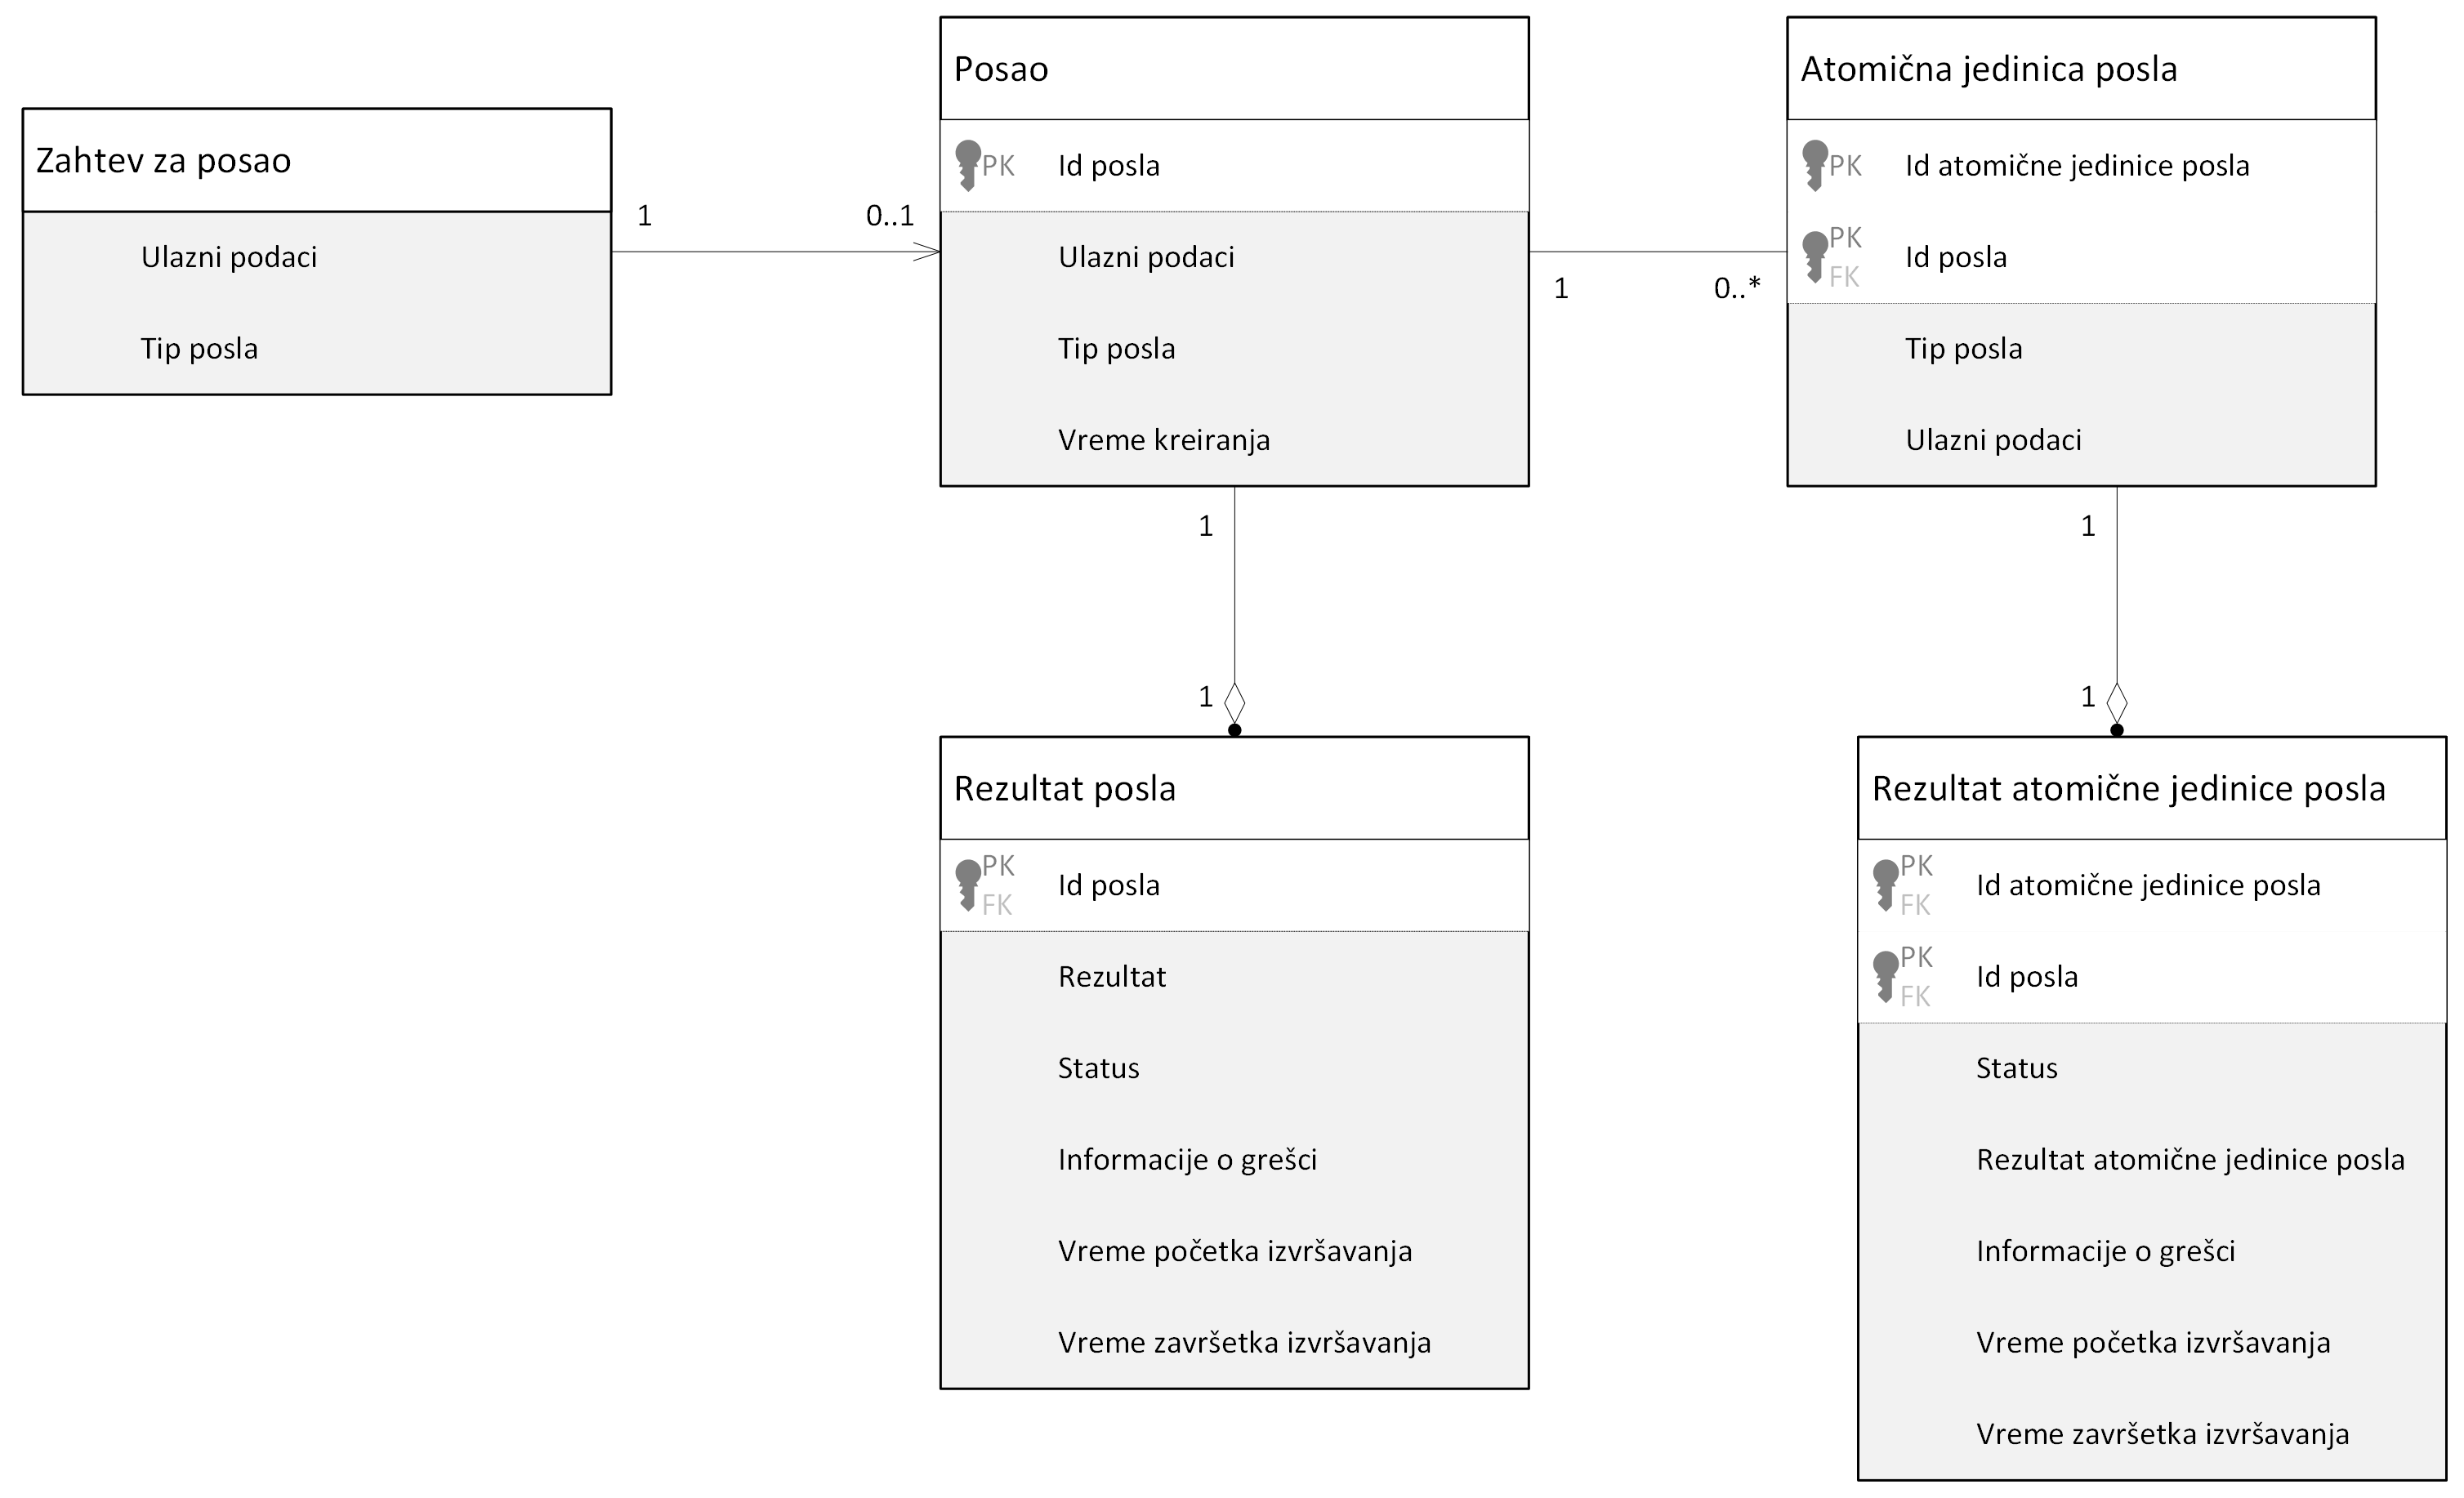
\includegraphics[width=1.0\textwidth]{./images/uml_er_dijagram_posao.png}
  \caption{ER dijagram entiteta - Posao}
  \label{fig:erposao}
\end{figure}



\section{Proces izvršavanja posla}
Stanja kroz koja prolazi posao su pikazana na slici \ref{fig:stanjaposla}.

\begin{figure}[!ht]
  \centering
  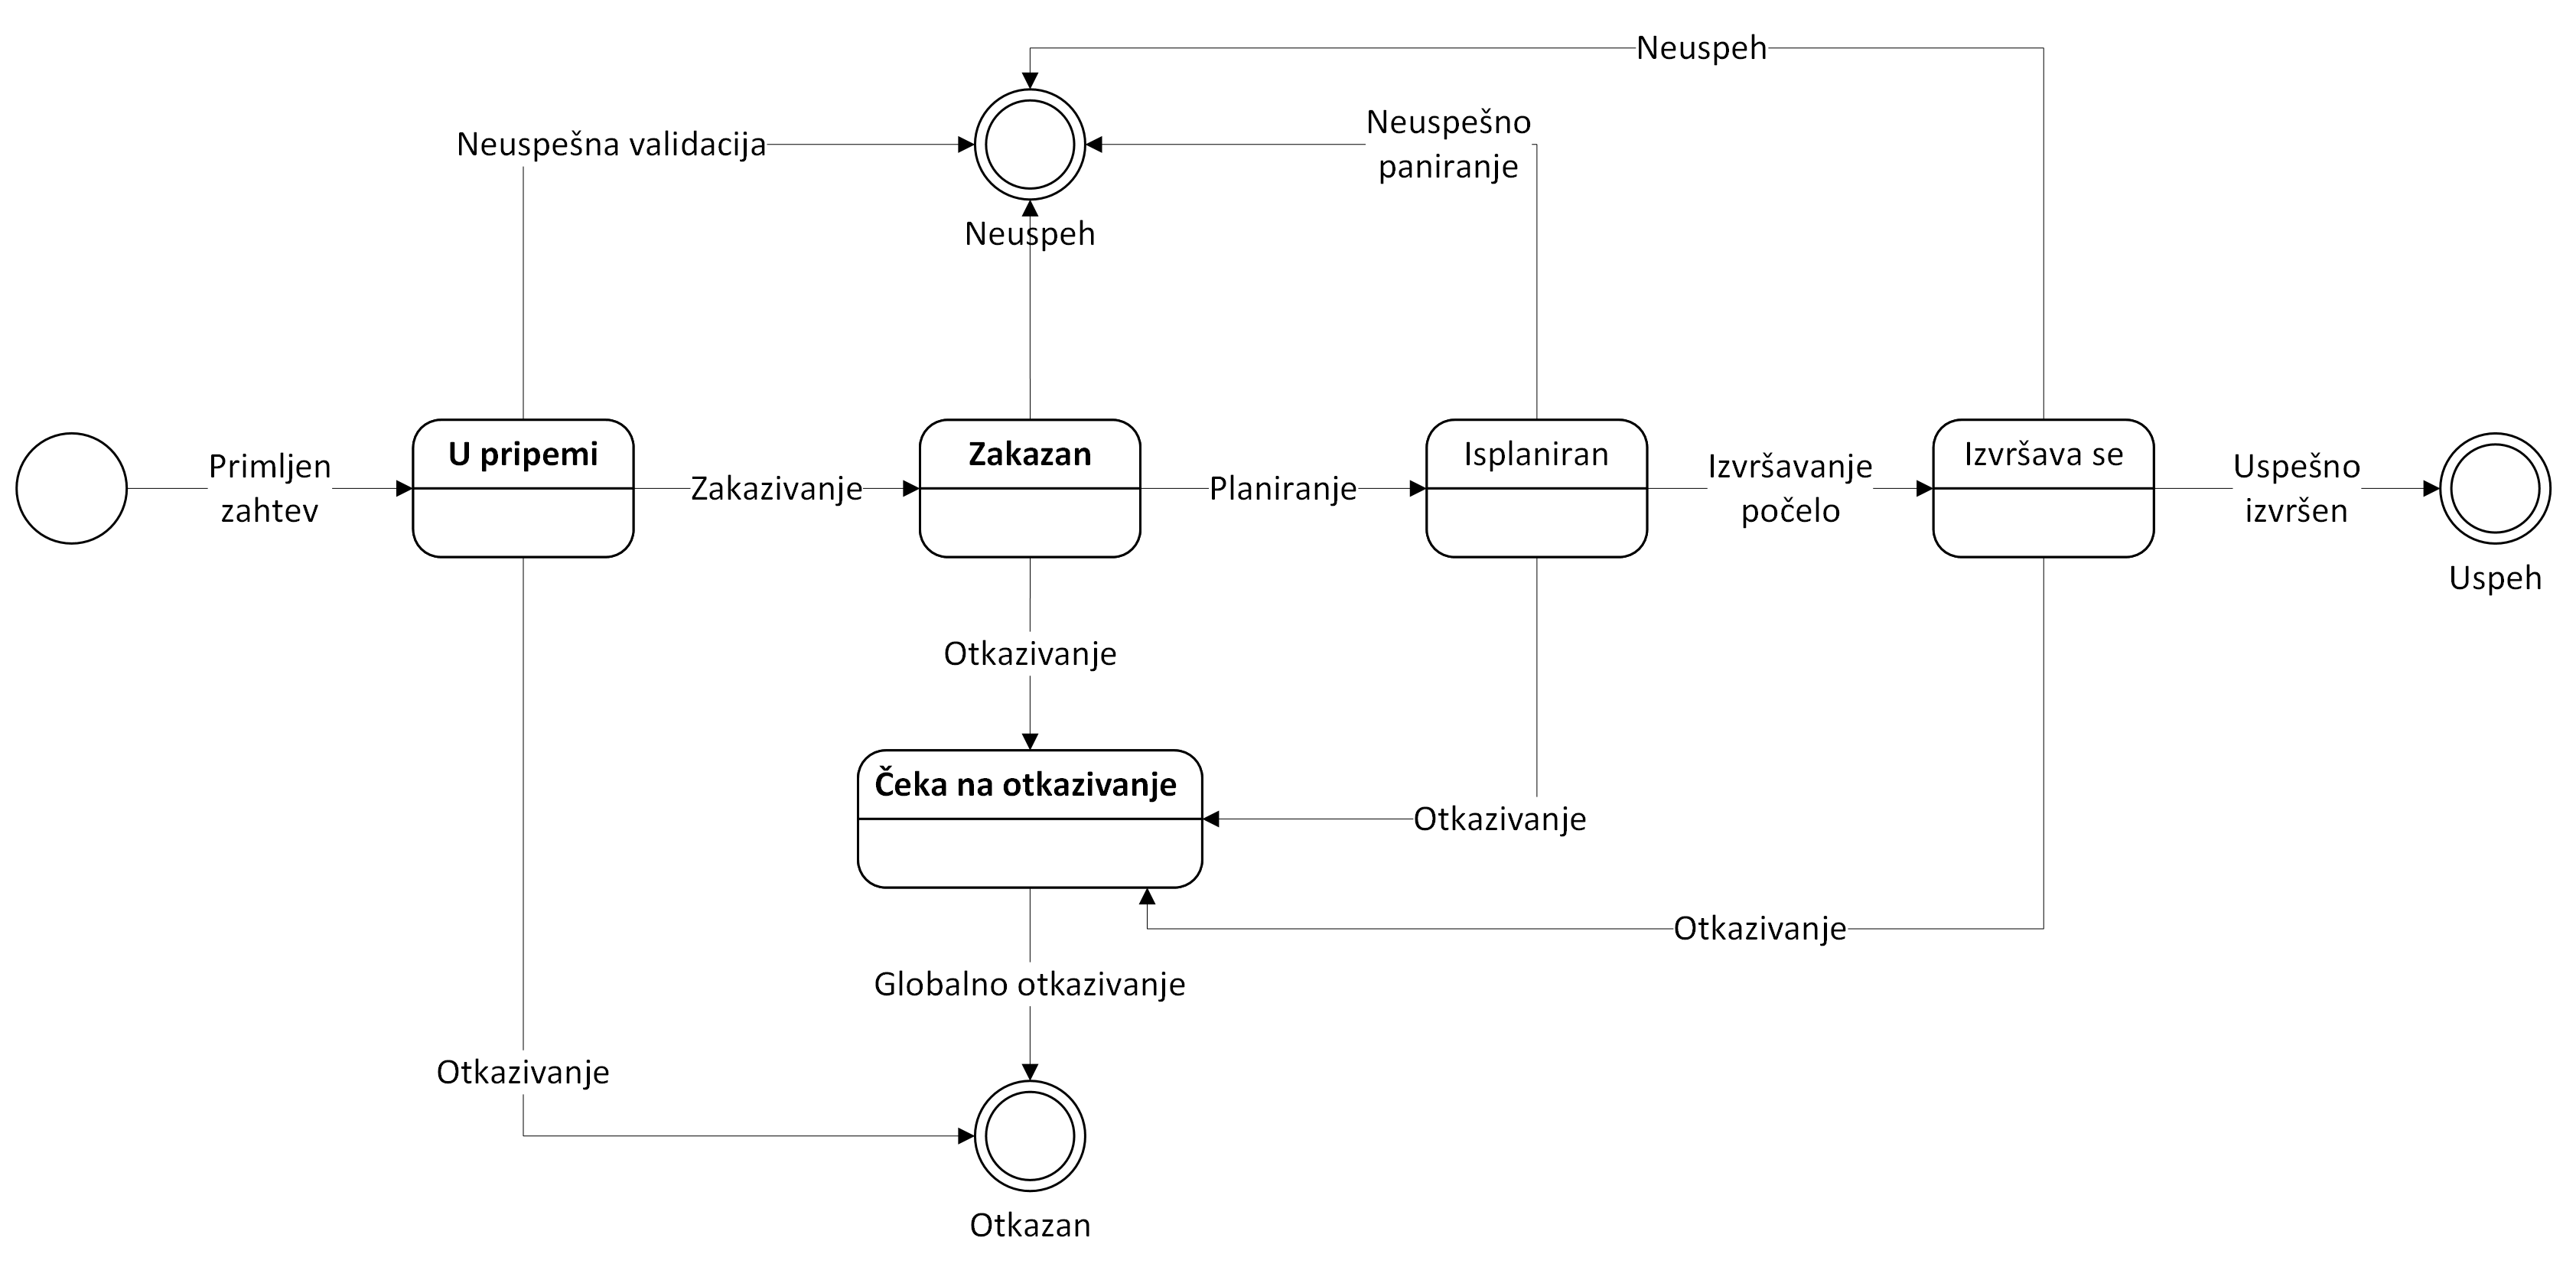
\includegraphics[width=1.0\textwidth]{./images/dijagram_stanja_posao.png}
  \caption{UML dijagram stanja - Posao}
  \label{fig:stanjaposla}
\end{figure}


\section{Distribuiranje atomičnih jedinica posla}
TODO

\section{Pokretanje u oblaku}
TODO

\subsection{Integracija sa Azure platformom}

U realizaciji je korišćena platforma \emph{Microsoft Azure} \cite{Azure}. Za upravljanje i pristup resursima u okviru ove platforme koristi se  \emph{Azure portal} \cite{AzurePortal}.

% ------------------------------------------------------------------------------
\chapter{Testiranje}
\label{chp:testiranjesistema}
% ------------------------------------------------------------------------------

U ovom poglavlju su opisani načini testiranja implementiranog sistema. Za izradu testova korišćen je \emph{XUnit} \cite{XUnit} radni okvir.

Svi testovi se nalaze na GitHub adresi projekta u \href{https://github.com/milana-kovacevic/DistributedComputationSystem/tree/main/tests}{tests} poddirektorijumu.

\emph{XUnit} radni okvir ima podršku za pisanje dva tipa testova: činjenice (eng. \emph{Fact}) i teorije (eng. \emph{Theory}). Činjenice su testovi koji ne primaju argumente, dok teorije predstavljaju paremetrizovane testove. Specifikacijom atributa iznad tela funkcije testa se definišu ulazi nad kojima se test pokreće, što značajno olakšava generisanje testova sa različitim ulazima.

Struktura foldera sa testovima je prikazana na slici \ref{fig:testovi}, a na slici \ref{fig:testexplorer} se nalazi vizuelni prikaz rezultata izvršavanja testova u okruženju \emph{Microsoft Visual Studio}.
% (TODO nova slika sa jos testova)

\begin{figure}[!ht]
  \centering
  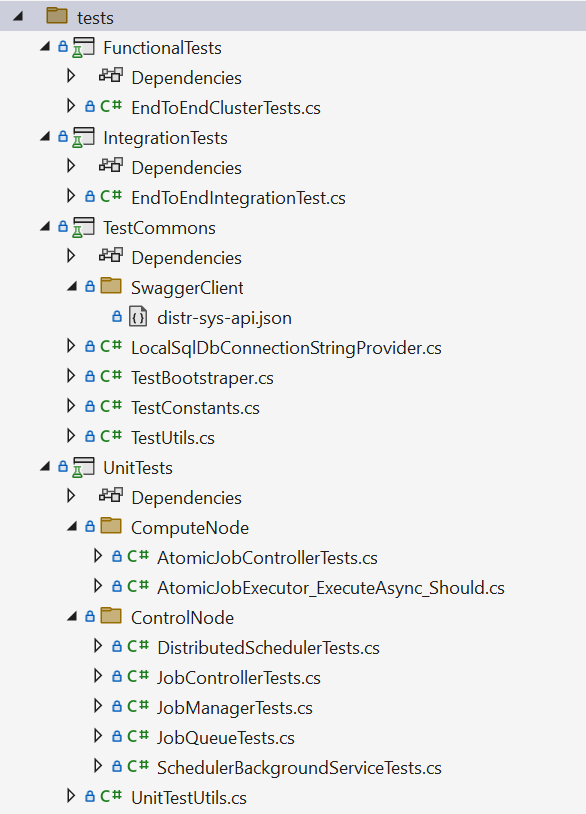
\includegraphics[width=0.8\textwidth]{./images/testovi.png}
  \caption{Struktura foldera sa testovima}
  \label{fig:testovi}
\end{figure}

\begin{figure}[!ht]
  \centering
  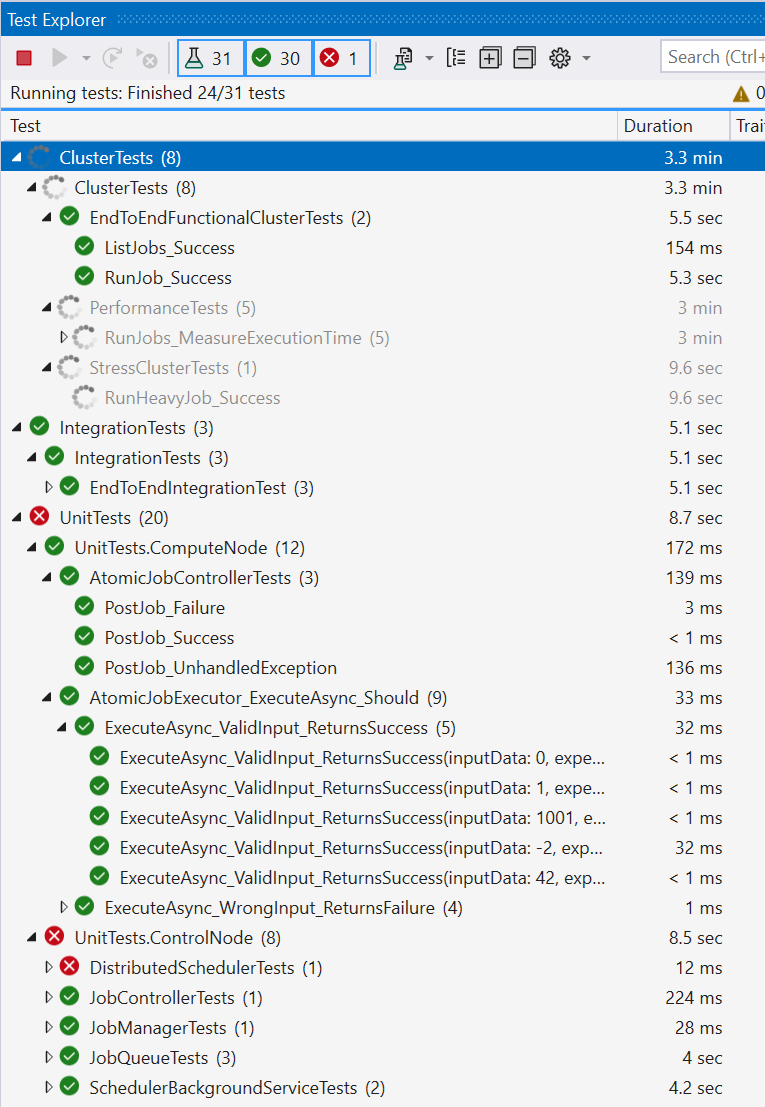
\includegraphics[width=0.8\textwidth]{./images/testexplorer.png}
  \caption{Pokretanje testova iz \emph{Test Explorer}-a u okruženju \emph{Microsoft Visual Studio}}
  \label{fig:testexplorer}
\end{figure}


%subfigures primer
%\begin{figure}[ht]
%\begin{subfigure}{.5\textwidth}
%  \centering
%  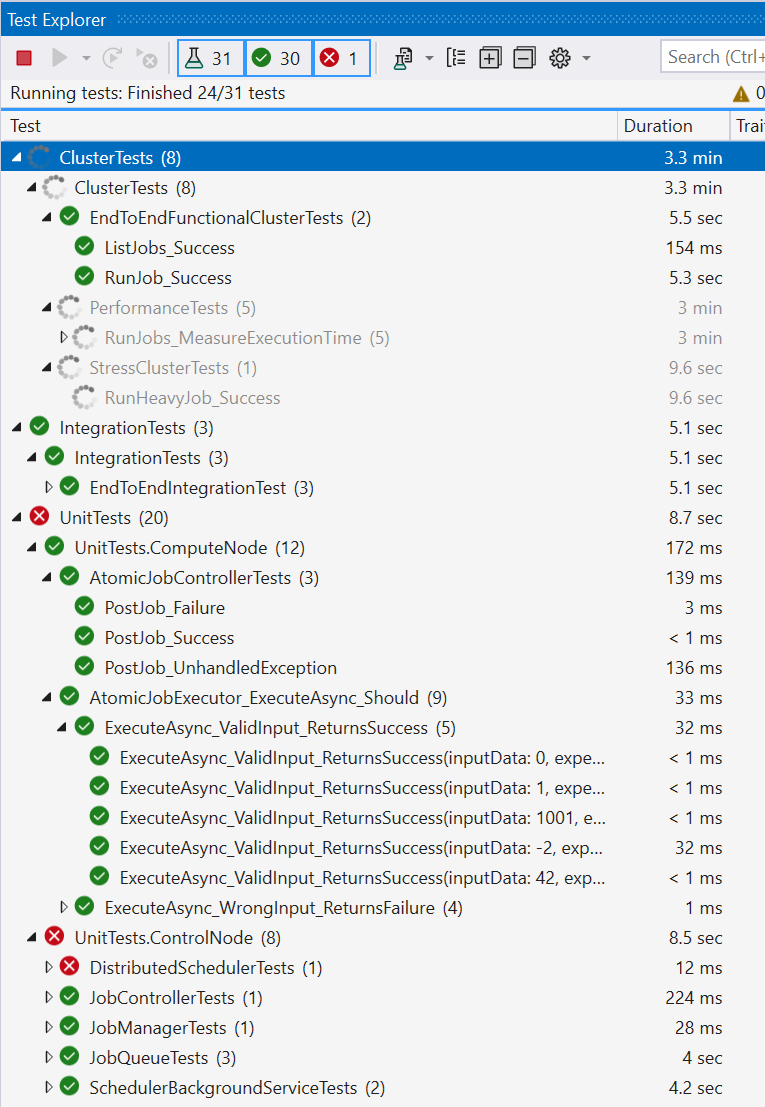
\includegraphics[width=1\textwidth]{./images/testexplorer.png}
%  \caption{Struktura foldera sa testovima}
%  \label{fig:testovi2}
%\end{subfigure}
%\begin{subfigure}{.5\textwidth}
%  \centering
%  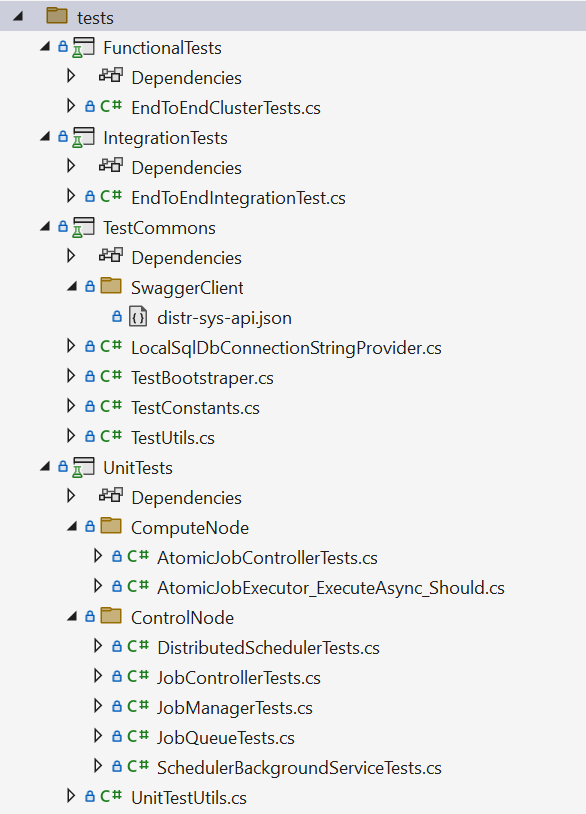
\includegraphics[width=1\textwidth]{./images/testovi.png}
%  \caption{Pokretanje testova iz \emph{Test Explorer}-a u okruženju \emph{Microsoft Visual Studio}}
%  \label{fig:testexplorer2}
%\end{subfigure}
%\caption{Put your caption here}
%\label{fig:fig}
%\end{figure}


Sistem je testiran na više nivoa, počevši od testiranja jedinica koda za svaku komponentu, zatim testova integracije, i, na najvišem nivou, funkcionalnih testova koji ukljucuju klaster testove.

\section{Testiranje jedinica koda}
Komponente \emph{Frontend} i \emph{ComputeNode} prate testovi jedinica koda. Testovi se nalaze u zasebnom projektu.
Tokom izrade testova jedinica koda, korišćen je radni okvir \emph{Moq} \cite{Moq} za mokovanje zavisnosti komponenata. U nastavku se nalazi slika \ref{fig:testscheduler} sa primerom testa jedinice koda.

\begin{figure}[h!]
\centering
\begin{lstlisting}
public class DistributedSchedulerTests
{
	private readonly ServiceProvider serviceProvider;
	private readonly Mock<IComputeNodeClientWrapper> mockedComputeNodeClient = new();

	public DistributedSchedulerTests()
	{
		var services = new ServiceCollection();
		services.AddSingleton<ILoggerFactory, LoggerFactory>();
		services.AddSingleton<ILogger<DistributedScheduler>, Logger<DistributedScheduler>>();

		// Setup mocked ComputeNodeClient
		mockedComputeNodeClient.Setup(m => m.RunAsync(It.IsAny<int>(), It.IsAny<int>(), It.IsAny<string>()))
			.Returns(Task.FromResult(new ComputeNodeSwaggerClient.AtomicJobResult()));
		services.AddScoped((services) => mockedComputeNodeClient.Object);

		services.AddScoped<IScheduler, DistributedScheduler>();

		serviceProvider = services.BuildServiceProvider();
	}

	[Fact]
	public async Task ScheduleJobAsync_Success()
	{
		var scheduler = serviceProvider.GetService<IScheduler>();
		Assert.NotNull(scheduler);

		var jobToBeScheduled = UnitTestUtils.GetDummyJob();
		await scheduler.ScheduleJobAsync(jobToBeScheduled);

		mockedComputeNodeClient.Verify(client => client.RunAsync(It.IsAny<int>(), jobToBeScheduled.Id, It.IsAny<string>()), Times.AtLeastOnce());
		Assert.NotEmpty(scheduler.GetInProgressTasks());
	}
}
\end{lstlisting}
\caption{Primer testa koji koristi \emph{Moq} radni okvir}
\label{fig:testscheduler}
\end{figure}

\section{Integracioni testovi}
Integracioni testovi testiraju integraciju između komponenti sistema: \emph{Frontend}a i \emph{ComputeNode}-a.

\section{Funkcionalni testovi}
Funkcionalni testovi testiraju funkcionalnost sistema iz ugla korisnika. U ovim testovima koristi se automatski generisana klijentska klasa \emph{DistributedCalculationSystemClient} nastala korišćenjem \emph{Swagger} alata. Ova klasa šalje zahteve ka \emph{Frontend} servisu, a u telu testova se proverava da li je odgovor od sistema očekivan.

Funkcionalni testovi se dele na nekoliko grupa:
\begin{enumerate}
\item Testovi nad lokalnim okruženjem - Testiraju osnovne funkcionalnosti servisa, u razvojnom okruženju.
\item Testovi nad klasterom u oblaku - Testiraju osnovne funkcionalnosti servisa u produkcionom okruženju.
\item Stres testovi - Skup testova koji se izvršavaju kako bi se analiziralo i unapredilo ponašanje sistema pod pritiskom. 
\item Testovi performansi - Skup testova koji se pokreću nad servisom pokrenutim u oblaku, sa fokusom na praćenje vremena potrebnog da sistem odradi očekivani posao. Cilj ovog testiranje je uvid u performanse sistema u odnosu na resurse dodeljene klasteru.
\end{enumerate}

Stres testovi i testovi performansi ispituju granice sistema. Oni su neophodni kako bi se na vreme razumela i unapredila uska grla sistema, kao i da bi se razumele mogućnosti sistema u skladu sa dodeljenim resursima.

TODO evaluacija kada budem imala ove testove u zadovoljavajućoj formi

\subsection{Testovi performansi nad klasterom sa različitim konfiguracijama}
TODO


% ------------------------------------------------------------------------------
\chapter{Praćenje metrika sistema}
\label{chp:pracenjemetrika}
% ------------------------------------------------------------------------------

Praćenje metrika sistema TODO

% ------------------------------------------------------------------------------
\chapter{Dalji razvoj sistema}
\label{chp:daljirazvoj}

% ------------------------------------------------------------------------------

Dalji razvoj sistema TODO


% ------------------------------------------------------------------------------
\chapter{Zaključak}
% ------------------------------------------------------------------------------
Zaključak, TODO

% ------------------------------------------------------------------------------
% Literatura
% ------------------------------------------------------------------------------
\literatura

% ==============================================================================
% Završni deo teze i prilozi
\backmatter
% ==============================================================================

% ------------------------------------------------------------------------------
% Biografija kandidata
\begin{biografija}
  \textbf{Milana Kovačević} je rođena u Zrenjaninu, 29. novembra 1995. godine. Osnovno i srednje obrazovanje (Zrenjaninska gimnazija, prirodno-matematički smer) završila je u rodnom gradu, uz sticanje diplome "Vuk Karadžić". Takođe je završila nižu muzičku školu, instrument klavir.
2014. godine je upisala osnovne studije na modulu Informatika na Matematičkom fakultetu Univerziteta u Beogradu. Osnovne studije je završila 2017. godine sa prosečnom ocenom 9.86, kao primalac stipendije Dositeja. Master akademske studije upisala je 2017. godine takođe na Matematičkom fakultetu na modulu Informatika. Položila je sve ispite predviđene planom i programom master akademskih studija sa prosečnom ocenom 9.15.

Nakon završetka osnovnih studija, nastavlja da se paralelno razvija i u industriji, radom u kompaniji Microsoft. Tokom rada se susreće sa sistemima za obradu i čuvanje podataka u okviru Azure plaforme, a radom na jednom od njih stiče i praktično znanje o distribuiranim sistemima i tehnologijama za rad u oblaku.

\end{biografija}
% ------------------------------------------------------------------------------

\end{document}
